\chapter{Text}
\label{ch:text}

As mentioned repeatedly, linguistic corpora, by their nature, consist of word forms, while other levels of linguistic representation are not represented unless the corresponding annotations \is{annotation} are added. In written \is{medium} corpora, there is one level other than the lexical that is (or can be) directly represented: the text. Well\hyp{}constructed linguistic corpora typically consist of (samples from) individual texts, whose meta\hyp{}information (author, title, original place and context of publication, etc.) are known. There is a substantial body of corpus\hyp{}linguistic research based on designs \is{research design} that combine the two inherently represented variables \textsc{Word (Form)} and \textsc{Text}; such designs may be concerned with the occurrence of words in individual texts, or, more typically, with the occurrence of words in clusters of texts belonging to the same language variety \is{language variety} (defined by topic, genre, \is{genre} function, etc.).

Texts are, of course, produced by speakers, and depending on how much and what kind of information about these speakers is available, we can also cluster texts according to demographic \is{demography} variables such as dialect, socioeconomic status, gender, age, \is{age} political or religious affiliation, etc. (as we have done in many of the examples in earlier chapters). In these cases, quantitative \is{quantitative research} corpus linguistics is essentially a variant of sociolinguistics, \is{sociolinguistics} differing mainly in that the linguistic phenomena it pays most attention to are not necessarily those most central to sociolinguistic \is{sociolinguistics} research in general.

\section{Keyword analysis}
\label{sec:keywordanalysis}

In the investigation of relationships between words (or other units of language structure) and texts (or clusters of texts), researchers frequently use a method referred to as \is{keyword analysis} \textit{keyword analysis}.\footnote{The term \textit{keyword} is frequently spelled as two words (\textit{key word}) or with a hyphen (\textit{key\hyp{}word}). I have chosen the spelling as a single word here because it seems simplest (at least to me, as a native writer of German, where compounds are always spelled as single words).} The term was originally used in contexts where cultural \is{culture} values and practices were studied through particular lexical items (cf. \citealt{williams_keywords:_1976}, \citealt{wierzbicka_cross-cultural_2003}); in corpus linguistics, it is used in a related but slightly broader sense of words that are characteristic of a particular text, language variety \is{language variety} or demographic \is{demography} in the sense that they occur with ``unusual frequency in a given text'' or set of texts, where ``unusual'' means high ``by comparison with a reference corpus of some kind'' \citep[236]{scott_pc_1997}.

In other words, the corpus\hyp{}linguistic identification of keywords \is{keyword analysis} is analogous to the identification of differential collocates, \is{collocation} except that it analyses the association \is{association} of a word W to a particular text (or collection of texts) T in comparison to the language as a whole (as represented by the reference corpus, which is typically a large, \is{corpus size} balanced corpus). \tabref{tab:keywordanalysis} shows this schematically.

\begin{table}
\caption{A generic 2\hyp{}by\hyp{}2 table for keyword analysis}
\label{tab:keywordanalysis}
\begin{tabular}[t]{llccc}
\lsptoprule
 & & \multicolumn{2}{c}{\textvv{Text}} & \\\cmidrule(lr){3-4}
 & & \textvv{text/corpus t} & \textvv{reference corpus} & Total \\
\midrule
\textvv{\makecell[lt]{Word}}
	& \textvv{word w}
		& \makecell[t]{O\textsubscript{11}}
		& \makecell[t]{O\textsubscript{12}}
		& \makecell[t]{R\textsubscript{1}} \\
	& \textvv{other words}
		& \makecell[t]{O\textsubscript{21}}
		& \makecell[t]{O\textsubscript{22}}
		& \makecell[t]{R\textsubscript{2}} \\
\midrule
	& Total
		& \makecell[t]{C\textsubscript{1}}
		& \makecell[t]{C\textsubscript{2}}
		& \makecell[t]{N} \\
\lspbottomrule
\end{tabular}
\end{table}

Just like collocation \is{collocation} analysis, keyword \is{keyword analysis} analysis is most often applied inductively, \is{induction} but there is nothing that precludes a deductive \is{deduction} design \is{research design} if we have hypotheses about the over- or underrepresentation of particular lexical items in a particular text or collection of texts. In either case, we have two nominal \is{nominal data} variables: \textsc{Keyword} (with the individual \textsc{words} as values) and \textsc{Text} (with the values \textsc{text} and \textsc{reference corpus}).

If keyword \is{keyword analysis} analysis is applied to a single text, the aim is typically to identify either the topic area or some stylistic \is{style} property of that text. When applied to text categories, the aim is typically to identify general lexical and\slash or grammatical \is{grammar} properties of the language variety \is{language variety} represented by the text categories.

As a first example of the kind of results that keyword \is{keyword analysis} analysis yields, consider \tabref{tab:threetextsfreq}, which shows the 20 most frequent tokens \is{token (instance)} (including punctuation marks) in the LOB \is{LOB} corpus and two individual texts (all words were converted to lower case).\largerpage

\begin{table}
\caption{Most frequent words in three texts (relative frequencies)}
\label{tab:threetextsfreq}
\resizebox{.7\textwidth}{!}{%
\begin{tabular}[t]{lr|lr|lr}
\lsptoprule
\multicolumn{2}{c|}{\textvv{LOB}} & \multicolumn{2}{c|}{\textvv{Text A}} & \multicolumn{2}{c}{\textvv{Text B}} \\
\midrule
\textit{the} & \num[round-mode=places,round-precision=6]{0.0590} & \textit{the} & \num[round-mode=places,round-precision=6]{0.0610} & \textit{the} & \num[round-mode=places,round-precision=6]{0.0585} \\
\textit{,} & \num[round-mode=places,round-precision=6]{0.0471} & \textit{,} & \num[round-mode=places,round-precision=6]{0.0584} & \textit{.} & \num[round-mode=places,round-precision=6]{0.0560} \\
\textit{.} & \num[round-mode=places,round-precision=6]{0.0435} & \textit{.} & \num[round-mode=places,round-precision=6]{0.0449} & \textit{,} & \num[round-mode=places,round-precision=6]{0.0452} \\
\textit{of} & \num[round-mode=places,round-precision=6]{0.0309} & \textit{in} & \num[round-mode=places,round-precision=6]{0.0383} & \textit{of} & \num[round-mode=places,round-precision=6]{0.0258} \\
\textit{and} & \num[round-mode=places,round-precision=6]{0.0241} & \textit{of} & \num[round-mode=places,round-precision=6]{0.0340} & \textit{a} & \num[round-mode=places,round-precision=6]{0.0231} \\
\textit{to} & \num[round-mode=places,round-precision=6]{0.0231} & \textit{and} & \num[round-mode=places,round-precision=6]{0.0256} & \textit{to} & \num[round-mode=places,round-precision=6]{0.0208} \\
\textit{a} & \num[round-mode=places,round-precision=6]{0.0197} & \textit{$($} & \num[round-mode=places,round-precision=6]{0.0137} & \textit{he} & \num[round-mode=places,round-precision=6]{0.0192} \\
\textit{in} & \num[round-mode=places,round-precision=6]{0.0184} & \textit{$)$} & \num[round-mode=places,round-precision=6]{0.0137} & \textit{``} & \num[round-mode=places,round-precision=6]{0.0150} \\
\textit{that} & \num[round-mode=places,round-precision=6]{0.0098} & \textit{at} & \num[round-mode=places,round-precision=6]{0.0123} & \textit{''} & \num[round-mode=places,round-precision=6]{0.0149} \\
\textit{is} & \num[round-mode=places,round-precision=6]{0.0096} & \textit{a} & \num[round-mode=places,round-precision=6]{0.0119} & \textit{and} & \num[round-mode=places,round-precision=6]{0.0148} \\
\textit{was} & \num[round-mode=places,round-precision=6]{0.0092} & \textit{to} & \num[round-mode=places,round-precision=6]{0.0117} & \textit{his} & \num[round-mode=places,round-precision=6]{0.0140} \\
\textit{it} & \num[round-mode=places,round-precision=6]{0.0091} & \textit{was} & \num[round-mode=places,round-precision=6]{0.0116} & \textit{was} & \num[round-mode=places,round-precision=6]{0.0138} \\
\textit{`} & \num[round-mode=places,round-precision=6]{0.0087} & \textit{neosho} & \num[round-mode=places,round-precision=6]{0.0112} & \textit{in} & \num[round-mode=places,round-precision=6]{0.0112} \\
\textit{'} & \num[round-mode=places,round-precision=6]{0.0085} & \textit{were} & \num[round-mode=places,round-precision=6]{0.0110} & \textit{that} & \num[round-mode=places,round-precision=6]{0.0110} \\
\textit{for} & \num[round-mode=places,round-precision=6]{0.0080} & \textit{species} & \num[round-mode=places,round-precision=6]{0.0078} & \textit{had} & \num[round-mode=places,round-precision=6]{0.0099} \\
\textit{he} & \num[round-mode=places,round-precision=6]{0.0078} & \textit{station} & \num[round-mode=places,round-precision=6]{0.0071} & \textit{hume} & \num[round-mode=places,round-precision=6]{0.0081} \\
\textit{i} & \num[round-mode=places,round-precision=6]{0.0066} & \textit{river} & \num[round-mode=places,round-precision=6]{0.0067} & \textit{on} & \num[round-mode=places,round-precision=6]{0.0078} \\
\textit{as} & \num[round-mode=places,round-precision=6]{0.0063} & \textit{that} & \num[round-mode=places,round-precision=6]{0.0065} & \textit{it} & \num[round-mode=places,round-precision=6]{0.0068} \\
\textit{with} & \num[round-mode=places,round-precision=6]{0.0062} & \textit{by} & \num[round-mode=places,round-precision=6]{0.0064} & \textit{--} & \num[round-mode=places,round-precision=6]{0.0063} \\
\textit{be} & \num[round-mode=places,round-precision=6]{0.0062} & \textit{1959} & \num[round-mode=places,round-precision=6]{0.0062} & \textit{as} & \num[round-mode=places,round-precision=6]{0.0063} \\
\lspbottomrule
\end{tabular}}
\end{table}
% me: all tokens, case insensitive

As we can see, the differences are relatively small, as all lists are dominated by frequent function words and punctuation marks. Ten of these occur on all three lists (\textit{a}, \textit{and}, \textit{in}, \textit{of}, \textit{that}, \textit{the}, \textit{to}, \textit{was}, the comma and the period), and another six occur on two of them (\textit{as}, \textit{he}, \textit{it}, \textit{on}, and opening and closing quotation marks -- although the latter are single quotation marks in the case of LOB \is{LOB} and double quotation marks in the case of Text B). Even the types \is{type (category)} that occur only once are mostly uninformative with respect to the language variety \is{language variety} (or text category) we may be dealing with (\textit{1959}, \textit{at}, \textit{by}, \textit{for}, \textit{had}, \textit{is}, \textit{with}, the hyphen and opening and closing parentheses). The only exceptions are four content words in Text A: \textit{Neosho}, \textit{river}, \textit{species}, \textit{station} -- these suggest that the text is about the \textit{Neosho} river and perhaps that it deals with biology (as suggested by the word \textit{species}).

Applying keyword \is{keyword analysis} analysis to each text or collection of texts allows us to identify the words that differ most significantly in frequency from the reference corpus, telling us how the text in question differs lexically from the (written) \is{medium} language of its time as a whole. \tabref{tab:fishreportkey} lists the keywords \is{keyword analysis} for Text A.

\begin{table}[t]
\caption{Keywords in a report on fish populations}
\label{tab:fishreportkey}
\resizebox{\textwidth}{!}{%
\begin{tabular}[t]{l S[table-format=3] S[table-format=4] S[table-format=5] S[table-format=7] S[table-format=3.2]}
\lsptoprule
\multicolumn{1}{c}{\makecell[tc]{\textvv{Keyword}}} & \multicolumn{1}{c}{\makecell[tc]{Frequency \\ in \textvv{report}}} & \multicolumn{1}{c}{\makecell[tc]{Frequency \\ in \textvv{LOB}}} & \multicolumn{1}{c}{\makecell[tc]{Other words \\ in \textvv{report}}} & \multicolumn{1}{c}{\makecell[tc]{Other words \\ in \textvv{LOB}}} & \multicolumn{1}{c}{\makecell[tc]{\emph{G}}} \\
\midrule
\textit{neosho} & 277 & 0 & 24525 & 1157496 & 2143.85754676855 \\
\textit{species} & 194 & 25 & 24608 & 1157471 & 1346.34569133827 \\
\textit{station} & 177 & 119 & 24625 & 1157377 & 975.304736947018 \\
\textit{river} & 165 & 104 & 24637 & 1157392 & 921.714686756413 \\
\textit{1957} & 137 & 57 & 24665 & 1157439 & 827.015414144296 \\
\textit{1959} & 153 & 124 & 24649 & 1157372 & 807.663174449525 \\
\textit{kansas} & 107 & 2 & 24695 & 1157494 & 807.539431152387 \\
\textit{cygnes} & 94 & 0 & 24708 & 1157496 & 726.835944146123 \\
\textit{marais} & 94 & 1 & 24708 & 1157495 & 715.780996710436 \\
\textit{catfish} & 90 & 0 & 24712 & 1157496 & 695.892508588732 \\
\textit{des} & 97 & 29 & 24705 & 1157467 & 615.323312002121 \\
\textit{fish} & 121 & 121 & 24681 & 1157375 & 605.360202906426 \\
\textit{upper} & 103 & 61 & 24699 & 1157435 & 582.56385976272 \\
\textit{abundance} & 81 & 7 & 24721 & 1157489 & 577.702494651473 \\
\textit{$($} & 340 & 2902 & 24462 & 1154594 & 577.40748732819 \\
\textit{$)$} & 340 & 2926 & 24462 & 1154570 & 573.116609220526 \\
\textit{channel} & 88 & 22 & 24714 & 1157474 & 571.2623085742 \\
\textit{shiner} & 75 & 3 & 24727 & 1157493 & 554.561054361179 \\
\textit{lower} & 103 & 120 & 24699 & 1157376 & 493.684469416984 \\
\textit{minnow} & 63 & 1 & 24739 & 1157495 & 476.7977064622 \\
\lspbottomrule
\end{tabular}}
\end{table}
% me: LOB_LEGACY vs. FISHREPORT, all tokens, case insensitive

The keywords \is{keyword analysis} now convey a very specific idea of what the text is about: there are two proper names of rivers (the \textit{Neosho} already seen on the frequency \is{frequency} list and the \textit{Marais des Cygnes}, represented by its constituents \textit{Cygnes}, \textit{Marais} and \textit{des}), and there are a number of words for specific species of fish as well as the words \textit{river} and \textit{channel}.

The text is clearly about fish in the two rivers. The occurrence of the words \textit{station} and \textit{abundance} suggests a research context, which is supported by the occurrence of two dates and opening and closing parentheses (which are often used in scientific texts to introduce references). The text in question is indeed a scientific report on fish populations: \textit{Fish Populations, Following a Drought, In the Neosho and Marais des Cygnes Rivers of Kansas} (available via Project Gutenberg and in the Supplementary Online Material, file TXQP). Note that the occurrence of some tokens \is{token (instance)} (such as the dates and the parentheses) may be characteristic of a language variety \is{language variety} rather than an individual text, a point we will return to below.\largerpage[-1]

Next, consider \tabref{tab:scifikey}, which lists the keywords \is{keyword analysis} for Text B. Three things are noticeable: the keyness \is{keyness} of a number of words that are most likely proper names (\textit{Hume}, \textit{Vye}, \textit{Rynch}, \textit{Wass}, \textit{Brodie} and \textit{Jumala}), pronouns \is{pronoun} (\textit{he}, \textit{his}) and punctuation marks indicative of direct speech (the quotation marks and the exclamation mark).\largerpage[-1]

\begin{table}[t]
\caption{Keywords in a science fiction novel}
\label{tab:scifikey}
\resizebox{\textwidth}{!}{%
\begin{tabular}[t]{l S[table-format=4] S[table-format=5] S[table-format=5] S[table-format=7] S[table-format=4.2]}
\lsptoprule
\multicolumn{1}{c}{\makecell[tc]{\textvv{Keyword}}} & \multicolumn{1}{c}{\makecell[tc]{Frequency \\ in \textvv{novel}}} & \multicolumn{1}{c}{\makecell[tc]{Frequency \\ in \textvv{LOB}}} & \multicolumn{1}{c}{\makecell[tc]{Other words \\ in \textvv{novel}}} & \multicolumn{1}{c}{\makecell[tc]{Other words \\ in \textvv{LOB}}} & \multicolumn{1}{c}{\makecell[tc]{\emph{G}}} \\
\midrule
\textit{``} & 604 & 77 & 24198 & 1157419 & 4205.14307110206 \\
\textit{''} & 601 & 121 & 24201 & 1157375 & 4011.51063154168 \\
\textit{hume} & 325 & 2 & 24477 & 1157494 & 2491.68595753249 \\
\textit{--} & 254 & 0 & 24548 & 1157496 & 1965.61541621278 \\
\textit{vye} & 228 & 0 & 24574 & 1157496 & 1764.1751305293 \\
\textit{rynch} & 134 & 0 & 24668 & 1157496 & 1036.34007757997 \\
\textit{.} & 2252 & 50324 & 22550 & 1107172 & 1000.71159535114 \\
\textit{he} & 772 & 9068 & 24030 & 1148428 & 952.737784983041 \\
\textit{wass} & 100 & 0 & 24702 & 1157496 & 773.253475159535 \\
\textit{his} & 565 & 6272 & 24237 & 1151224 & 740.624919140107 \\
\textit{'s} & 214 & 1177 & 24588 & 1156319 & 510.858785197556 \\
\textit{the} & 2352 & 68350 & 22450 & 1089146 & 475.704566275507 \\
\textit{had} & 397 & 5473 & 24405 & 1152023 & 398.127782320442 \\
\textit{brodie} & 44 & 0 & 24758 & 1157496 & 340.13407369537 \\
\textit{was} & 556 & 10685 & 24246 & 1146811 & 327.11360582672 \\
\textit{,} & 1820 & 54548 & 22982 & 1102948 & 319.741050413579 \\
\textit{flitter} & 41 & 0 & 24761 & 1157496 & 316.938253211963 \\
\textit{a} & 931 & 22857 & 23871 & 1134639 & 313.15958677858 \\
\textit{hunter} & 43 & 12 & 24759 & 1157484 & 275.204326155239 \\
\textit{could} & 171 & 1741 & 24631 & 1155755 & 244.217436561136 \\
\lspbottomrule
\end{tabular}}
\end{table}
% me: LOB_LEGACY vs. STARHUNTER, all tokens, case insensitive

This does not tell us anything about this particular text, but taken together, these pieces of evidence point to a particular genre: \is{genre} narrative text (novels, \is{literary language} short stories, etc.). The few potential content words suggest a particular sub\hyp{}genre: the archaic \textit{hunter} in combination with the unusual word \textit{flitter} is suggestive of fantasy or science fiction. If we were to include the next twenty most strongly associated \is{association} nouns, \is{noun} we would find \textit{patrol}, \textit{camp}, \textit{needler}, \textit{safari}, \textit{guild}, \textit{tube}, \textit{planet} and \textit{out\hyp{}hunter}, which corroborate the impression that we are dealing with a science\hyp{}fiction \is{literary language} novel. And indeed, the text in question is the science\hyp{}fiction novel \textit{Starhunter} by Andre Alice Norton (available via Project Gutenberg in the Supplementary Online Material, file TXQP).

Again, the keywords \is{keyword analysis} identified are a mixture of topical markers and markers for the language variety \is{language variety} (in this case, the genre) \is{genre} of the text, so even a study of the keywords of single texts provides information about more general linguistic properties of the text in question as well as its specific topic. But keyword \is{keyword analysis} analysis reveals its true potential when we apply it to clusters of texts, as in the case studies in the next section.

\section{Case studies}\label{sec:keywordcasestudies}
\subsection{Language Variety}\label{sec:texttype}

Keyword \is{keyword analysis} analysis has been applied to a wide range of language varieties \is{language variety} defined by topic area (e.g. travel writing), genre \is{genre} (e.g. news reportage) \is{newspaper language} or both (e.g. history textbooks) (see the contributions in \citealt{bondi_keyness_2010} for recent examples). Here, we will look at two case studies of scientific language.

\subsubsection{Case study: Keywords in scientific writing}
\label{sec:keywordsinscientificwriting}

There are a number of keyword\hyp{}based \is{keyword analysis} analyses of academic \is{academic language} writing (cf., for example, \citealt{scott_textual_2006} on literary \is{literary language} criticism, \citealt{romer_applying_2010} on academic student essays). Instead of replicating \is{replicability} one of these studies in detail, let us look more generally at the Learned \is{academic language} and Scientific Writing section of the LOB \is{LOB} (Section J), using the rest of the corpus (all sections except Section J) as a reference corpus. \tabref{tab:learnedlobbkey} shows the keywords \is{keyword analysis} for this section.

\begin{table}
\caption{Key words in the Learned and Scientific Writing section of LOB}
\label{tab:learnedlobbkey}
\resizebox{\textwidth}{!}{%
\begin{tabular}[t]{l S[table-format=5] S[table-format=5] S[table-format=6] S[table-format=6] S[table-format=4.2]}
\lsptoprule
\multicolumn{1}{c}{\makecell[tc]{\textvv{Keyword}}} & \multicolumn{1}{c}{\makecell[tc]{Frequency \\ in \textvv{lob j}}} & \multicolumn{1}{c}{\makecell[tc]{Frequency in \\ \textvv{other sections}}} & \multicolumn{1}{c}{\makecell[tc]{Other words \\ in \textvv{lob j}}} & \multicolumn{1}{c}{\makecell[tc]{Other words in \\ \textvv{other sections}}} & \multicolumn{1}{c}{\makecell[tc]{\emph{G}}} \\
\midrule
\textit{of} & 7899 & 27846 & 173017 & 948734 & 1065.04638043146 \\
\textit{@} & 313 & 36 & 180603 & 976544 & 942.81564402586 \\
\textit{$($} & 1099 & 1803 & 179817 & 974777 & 844.527153580497 \\
\textit{$)$} & 1101 & 1825 & 179815 & 974755 & 834.66176070663 \\
\textit{the} & 13125 & 55225 & 167791 & 921355 & 666.504967418239 \\
\textit{=} & 102 & 3 & 180814 & 976577 & 352.442427273622 \\
\textit{is} & 2482 & 8619 & 178434 & 967961 & 348.237314932627 \\
\textit{in} & 4332 & 16917 & 176584 & 959663 & 345.369311367296 \\
\textit{fig} & 113 & 31 & 180803 & 976549 & 280.033479312755 \\
\textit{data} & 88 & 8 & 180828 & 976572 & 274.334471554413 \\
\textit{equation} & 72 & 0 & 180844 & 976580 & 267.285514550513 \\
\textit{values} & 111 & 47 & 180805 & 976533 & 235.702271725609 \\
\textit{oxygen} & 63 & 2 & 180853 & 976578 & 216.689012985925 \\
\textit{sodium} & 60 & 2 & 180856 & 976578 & 205.743466498154 \\
\textit{results} & 121 & 81 & 180795 & 976499 & 204.674997380884 \\
\textit{obtained} & 98 & 49 & 180818 & 976531 & 193.329942125712 \\
\textit{experiments} & 72 & 15 & 180844 & 976565 & 192.395828660292 \\
\textit{\%} & 77 & 22 & 180839 & 976558 & 188.442264502073 \\
\textit{model} & 83 & 33 & 180833 & 976547 & 180.801823144271 \\
\textit{solution} & 96 & 53 & 180820 & 976527 & 180.42840041207 \\
\lspbottomrule
\end{tabular}}
\end{table}
% me: LOB_LEGACY J against all other sections, all tokens, case insensitive

It is immediately obvious from the preponderance of scientific terminology that we are dealing with Scientific English -- there are general scientific terms like \textit{fig(ure)}, \textit{data} \textit{experiment} or \textit{model}, mathematical terms and symbols (\textit{equation}, \textit{values}, the equals and percent signs), and a few words from chemistry (\textit{oxygen}, \textit{sodium}) (the reason the @ sign appears on this list is because it is used to mark places in the corpus where material such as mathematical formulae and operators have been deleted).

It may not be surprising that scientific terminology dominates in a corpus of Scientific English, but it demonstrates that keyword \is{keyword analysis} analysis works. Given this, we can make some more profound observations on the basis of the list in \tabref{tab:learnedlobbkey}. For example, we observe that certain kinds of punctuation are typical of academic \is{academic language} writing in general (such as the parentheses, which we already suspected based on the analysis of the fish population report in Section~\ref{sec:keywordanalysis} above). Even more interestingly, keyword \is{keyword analysis} analysis can reveal function words that are characteristic for a particular language variety \is{language variety} and thus give us potential insights into grammatical \is{grammar} structures that may be typical for it; for example, \textit{is}, \textit{the} and \textit{of} are among the most significant keywords of Scientific English. The last two are presumably related to the \textit{nominal \is{noun} style} \is{style} that is known to characterize academic \is{academic language} texts, while the higher\hyp{}than\hyp{}normal frequency \is{frequency} of \textit{is} may be due to the prevalence of definitions, statements of equivalence, etc. This (and other observations made on the basis of keyword \is{keyword analysis} analysis) would of course have to be followed up by more detailed analyses of the function these words serve -- but keyword analysis tells us what words are likely to be interesting to investigate.

\subsubsection{Case study: [a + \_\_ + of] in Scientific English}
\label{sec:anofinmedicalresearchpapers}

Of course, keyword \is{keyword analysis} analysis is not the only way to study lexical characteristics of language varieties. \is{language variety} In principle, any design \is{research design} studying the interaction of lexical items with other units of linguistic structure can also be applied to specific language varieties.

For example, \citet{marco_collocational_2000} investigates collocational \is{collocation} frameworks \is{collocational framework} (see \chapref{ch:grammar}, Section~\ref{sec:collocationalframeworksandgrammarpatterns}) in medical research papers. While this may not sound particularly interesting at first glance, it turns out that even highly frequent frameworks like [\textit{a \_\_ of}] are filled by completely different items from those found in the language as a whole, which is important for many applied purposes (such as language teaching or machine processing of language), but which also shows just how different language varieties \is{language variety} can actually be. Since Marco's corpus is not publicly available and the Learned \is{academic language} and Scientific Writing section of LOB \is{LOB} is too small for this kind of analysis, let us use the Written Academic subsection of the BNC Baby. \is{BNC Baby} \tabref{tab:anoflearnedfreq} shows the 15 most strongly associated \is{association} collocates \is{collocation} in the framework \is{collocational framework} [\textit{a \_\_ of}], i.e. the words whose frequency \is{frequency} of occurrence inside this framework differs most significantly from their frequency of occurrence outside of this framework in the same corpus section.

\begin{table}
\caption{Collocates of the framework [\textit{a} \_\_ \textit{of}] in the Written Academic subsection of BNC Baby}
\label{tab:anoflearnedfreq}
\resizebox{\textwidth}{!}{%
\begin{tabular}[t]{l *{2}{S[table-format=3]} S[table-format=4] S[table-format=7] S[table-format=4.2]}
\lsptoprule
\multicolumn{1}{c}{\makecell[tc]{\textvv{Collocate}}} & \multicolumn{1}{c}{\makecell[tc]{Frequency in \\ $[$\textit{a} \_\_ \textit{of}$]$ }} & \multicolumn{1}{c}{\makecell[tc]{Frequency in \\ other contexts}} & \multicolumn{1}{c}{\makecell[tc]{Other words in \\ $[$\textit{a} \_\_ \textit{of}$]$}} & \multicolumn{1}{c}{\makecell[tc]{Other words in \\ other contexts}} & \multicolumn{1}{c}{\makecell[tc]{\emph{G}}} \\
\midrule
\textit{number} & 272 & 805 & 2965 & 1138862 & 2001.8435699171 \\
\textit{series} & 99 & 203 & 3138 & 1139464 & 783.667251087437 \\
\textit{variety} & 82 & 163 & 3155 & 1139504 & 652.774047772446 \\
\textit{result} & 98 & 425 & 3139 & 1139242 & 650.603952199947 \\
\textit{matter} & 61 & 190 & 3176 & 1139477 & 439.564574439839 \\
\textit{function} & 65 & 319 & 3172 & 1139348 & 416.521135032684 \\
\textit{range} & 66 & 388 & 3171 & 1139279 & 401.451789166953 \\
\textit{set} & 59 & 442 & 3178 & 1139225 & 332.637399492872 \\
\textit{lot} & 36 & 61 & 3201 & 1139606 & 295.189976627841 \\
\textit{form} & 65 & 933 & 3172 & 1138734 & 288.418237292356 \\
\textit{combination} & 34 & 115 & 3203 & 1139552 & 239.888093602344 \\
\textit{measure} & 35 & 139 & 3202 & 1139528 & 237.133277709872 \\
\textit{consequence} & 33 & 109 & 3204 & 1139558 & 234.178040913071 \\
\textit{piece} & 29 & 73 & 3208 & 1139594 & 219.153519937284 \\
\textit{group} & 43 & 605 & 3194 & 1139062 & 192.121246046857 \\
\textit{list} & 28 & 125 & 3209 & 1139542 & 183.847199884568 \\
\textit{source} & 26 & 161 & 3211 & 1139506 & 155.380824149027 \\
\textit{way} & 41 & 870 & 3196 & 1138797 & 152.056359343873 \\
\textit{study} & 36 & 594 & 3201 & 1139073 & 150.153705753867 \\
\textit{sense} & 29 & 294 & 3208 & 1139373 & 147.065016772325 \\
\lspbottomrule
\multicolumn{6}{l}{\scriptsize{Supplementary Online Material: FXHV}} \\ %OSM
\end{tabular}}
\end{table}
% me: collexeme analysis, case insensitive

If we compare the result in \tabref{tab:anoflearnedfreq} to that in \tabref{tab:axofcollframe} in \chapref{ch:grammar}, we notice clear differences between the use of this framework \is{collocational framework} in academic \is{academic language} texts and the language as a whole; for example, \textit{lot}, which is most strongly associated \is{association} with the framework in the general language occurs in 9th position, while the top collocates \is{collocation} of the framework \is{collocational framework} are more precise quantification \is{quantitative research} terms like \textit{number} or \textit{series}, and general scientific terms like \textit{result} and \textit{function}.

However, the two lists -- that in \tabref{tab:axofcollframe} and that presented here -- were derived independently from different corpora, making it difficult to determine the true extent of the differences. In particular, in each of the two corpora the words in the pattern compete with the words outside of the pattern, which are obviously from the same discourse domains. To get a clearer idea of the different function(s) that a pattern might play in two different language varieties, \is{language variety} we can combine collocational \is{collocation} framework \is{collocational framework} analysis and keyword \is{keyword analysis} analysis: we extract \is{retrieval} all words occurring in a collocational framework (or grammar \is{grammar} pattern, \is{grammar pattern} construction, etc.) in a particular language variety, \is{language variety} and compare them to the words occurring in the same pattern in a reference corpus (\citealt{stefanowitsch_lot_2017} refers to this mix of keyword \is{keyword analysis} and collostructional \is{collostructional analysis} analysis as ``textually\hyp{}distinctive [i.e., differential] collexeme \is{collexeme!differential} analysis'').

\tabref{tab:anoflearnedkey} shows the result of such an analysis in the BNC Baby, \is{BNC Baby} comparing words occurring in the framework \is{collocational framework} [\textit{a(n)} \_ \textit{of}] in the Written Academic \is{academic language} section to the words occurring in the same pattern in the rest of the corpus (all sections other than Written Academic).

\begin{table}
\caption{Textually differential collexemes in the framework $[$\textit{a} + \_ + \textit{of}$]$ in the Written Academic section of BNC Baby compared to all other sections}
\label{tab:anoflearnedkey}
\resizebox{\textwidth}{!}{%
\begin{tabular}[t]{l *{2}{S[table-format=3]} *{2}{S[table-format=7]} S[table-format=3.2]}
\lsptoprule
\multicolumn{1}{c}{\makecell[tc]{\textvv{Keyword}}} & \multicolumn{1}{c}{\makecell[tc]{Frequency in \\ $[$\textit{a} + \_ + \textit{of}$]$ \\ in Wrt. Acad.}} & \multicolumn{1}{c}{\makecell[tc]{Frequency in \\ $[$\textit{a} + \_ + \textit{of}$]$ \\ in other sections}} & \multicolumn{1}{c}{\makecell[tc]{Frequency in \\ other contexts \\ in Wrt. Acad.}} & \multicolumn{1}{c}{\makecell[tc]{Frequency in \\ other contexts \\ in other sections}} & \multicolumn{1}{c}{\makecell[tc]{\emph{G}}} \\
\midrule
\textit{number} & 272 & 151 & 1139395 & 3505016 & 298.079769744575 \\
\textit{function} & 65 & 0 & 1139602 & 3505167 & 182.65533525054 \\
\textit{form} & 65 & 17 & 1139602 & 3505150 & 108.524115849062 \\
\textit{variety} & 82 & 35 & 1139585 & 3505132 & 107.360346596459 \\
\textit{range} & 66 & 20 & 1139601 & 3505147 & 103.441601338926 \\
\textit{result} & 98 & 64 & 1139569 & 3505103 & 94.0314553677179 \\
\textit{series} & 99 & 81 & 1139568 & 3505086 & 76.0732182844072 \\
\textit{study} & 36 & 6 & 1139631 & 3505161 & 70.0906119931282 \\
\textit{measure} & 35 & 6 & 1139632 & 3505161 & 67.592867724927 \\
\textit{consequence} & 33 & 5 & 1139634 & 3505162 & 65.9544448366265 \\
\textit{set} & 59 & 32 & 1139608 & 3505135 & 65.7910710487631 \\
\textit{solution} & 23 & 0 & 1139644 & 3505167 & 64.6312481948337 \\
\textit{critique} & 23 & 1 & 1139644 & 3505166 & 56.8804233749769 \\
\textit{theory} & 20 & 0 & 1139647 & 3505167 & 56.2010456562647 \\
\textit{process} & 26 & 5 & 1139641 & 3505162 & 48.4847755359066 \\
\textit{matrix} & 17 & 0 & 1139650 & 3505167 & 47.7708550375946 \\
\textit{feature} & 15 & 0 & 1139652 & 3505167 & 42.1507345802581 \\
\textit{breach} & 19 & 2 & 1139648 & 3505165 & 41.3083621307484 \\
\textit{combination} & 34 & 16 & 1139633 & 3505151 & 41.863489729928 \\
\textit{consideration} & 14 & 0 & 1139653 & 3505167 & 39.3406763372276 \\
\lspbottomrule
\multicolumn{6}{l}{\scriptsize{Supplementary Online Material: MPXF}} \\ %OSM
\end{tabular}}
\end{table}
% me: distinctive textual collexeme analysis, case insensitive

The scientific vocabulary now dominates the collocates \is{collocation} of the framework even more clearly than in the simple collocational framework \is{collocational framework} analysis above: the informal \textit{a lot of} and other colloquial words are now completely absent. This case study shows the variability that even seemingly simple grammatical \is{grammar} patterns may display across language varieties. \is{language variety} It is also meant to demonstrate how simple techniques like collocational\hyp{}framework \is{collocation} analysis can be combined with more sophisticated techniques to yield more insightful results.

\subsection{Comparing speech communities}
\label{sec:comparingspeechcommunities}

As pointed out at the beginning of this chapter, a keyword \is{keyword analysis} analysis of corpora that are defined by demographic \is{demography} variables is essentially a variant of variationist \is{variation} sociolinguistics. \is{sociolinguistics} The basic method remains the same, the only difference being that the corpora under investigation have to be constructed based on the variables in question, or, more typically, that existing corpora have to be separated into subcorpora accordingly. This is true for inductive \is{induction} keyword analyses as well as for the kind of deductive \is{deduction} analysis of individual words or constructions that we used in some of the examples in earlier chapters. The dependent variable will, as in all examples in this and the preceding chapter, always be nominal, \is{nominal data} consisting of (some part of) the lexicon \is{lexicon} (with words as values).

Lectal variety \is{language variety} (dialect, sociolect, etc.) is an obvious demographic \is{demography} category to investigate using corpus\hyp{}linguistic methods. Language varieties \is{language variety} differ from each other along a number of dimensions, one of which is the lexicon. \is{lexicon} While lexical differences have not tended to play a major role in mainstream sociolinguistics, \is{sociolinguistics} they do play a role in corpus\hyp{}based sociolinguistics \is{sociolinguistics} -- presumably, because they are relatively easy to extract \is{retrieval} from appropriately constructed corpora, but also because they have traditionally been an important defining criterion of dialects (and continue to be so, especially in applied contexts).\pagebreak

Many of the examples in the early chapters of this book demonstrate how, in principle, lexical differences between varieties \is{language variety} can be investigated -- take two sufficiently large \is{corpus size} corpora representing two different varieties, and study the distribution \is{distribution!conditional} of a particular word across these two corpora. Alternatively, we can study the distribution of \textit{all} words across the two corpora in the same way as we studied their distribution across texts or language varieties in the preceding section.

This was actually done fairly early, long before the invention of keyword \is{keyword analysis} analysis, by \citet{johansson_frequency_1989}. They compare all word forms in the LOB \is{LOB} and BROWN \is{BROWN} corpora using a ``coefficient of difference'', essentially the percentage of the word in the two corpora.\footnote{More precisely, in its generalized form, this coefficient is calculated by the following formula, given two corpora A and B:

\[\frac{ \frac{f ( \text{word}_A )}{\text{size}_A} - \frac{f ( \text{word}_B )}{\text{size}_B}}{ \frac{f ( \text{word}_A )}{ \text{size}_A} + \frac{f ( \text{word}_B )}{\text{size}_B}}\]

This formula will give us the percentage of uses of the word in Corpus A or Corpus B (whichever is larger), with a negative sign if it occurs in Corpus B.} In addition, they test each difference for significance using the $\chi^2$ \is{chi-square test} test. As discussed in \chapref{ch:collocation}, it is more recommendable -- and, in fact, simpler -- to use an association \is{association} measure \is{association measure} like \emph{G} right away, as percentages will massively overestimate infrequent events (a word that occurs only a single time will be seen as 100 percent typical of whichever corpus it happens to occur in); also, the $\chi^2$ \is{chi-square test} test cannot be applied to infrequent words. Still, Johansson and Hofland's basic idea is highly innovative and their work constitutes the first example of a keyword \is{keyword analysis} analysis that I am aware of.

Comparing two (large) \is{corpus size} corpora representing two varieties \is{language variety} will not, however, straightforwardly result in a list of dialect differences. Instead, there are at least five types of differences that such a comparison will uncover. Not all of them will be relevant to a particular research design, \is{research design} and some of them are fundamental problems for any research design and must be dealt with before we can proceed.

\tabref{tab:breamekeyone} shows the ten most strongly differential keywords \is{keyword analysis} for the LOB \is{LOB} and BROWN \is{BROWN} corpora. The analysis is based on the tagged versions of the two corpora as originally distributed by ICAME.

\begin{table}
\caption{Key words of British and American English based on a comparison of LOB and BROWN}
\label{tab:breamekeyone}
\resizebox*{!}{\textheight}{%
\begin{tabular}[t]{l *{2}{S[table-format=4]} *{2}{S[table-format=7]} S[table-format=6.2]}
\lsptoprule
\multicolumn{1}{c}{\makecell[tc]{\textvv{Keyword}}} & \multicolumn{1}{c}{\makecell[tc]{Frequency \\ in BROWN}} & \multicolumn{1}{c}{\makecell[tc]{Frequency \\ in LOB}} & \multicolumn{1}{c}{\makecell[tc]{Other words \\ in BROWN}} & \multicolumn{1}{c}{\makecell[tc]{Other words \\ in LOB}} & \multicolumn{1}{c}{\makecell[tc]{\emph{G}}} \\
\midrule
\multicolumn{6}{l}{Most strongly associated with \textvv{american english}} \\
\midrule
\textit{--} & 3385 & 0 & 1134081 & 1157496 & 4757.04131405291 \\
\textit{J} & 1776 & 128 & 1135690 & 1157368 & 1731.31166345718 \\
\textit{Mr.} & 851 & 0 & 1136615 & 1157496 & 1194.97768187181 \\
\textit] & 798 & 0 & 1136668 & 1157496 & 1120.53609787255 \\
\textit{F} & 1017 & 102 & 1136449 & 1157394 & 884.663049472858 \\
\textit{Mrs.} & 534 & 0 & 1136932 & 1157496 & 749.769879701268 \\
\textit{don't} & 489 & 0 & 1136977 & 1157496 & 686.577263054858 \\
\textit{The} & 455 & 0 & 1137011 & 1157496 & 638.832922248561 \\
\textit{didn't} & 402 & 0 & 1137064 & 1157496 & 564.409966174308 \\
\textit{program} & 376 & 0 & 1137090 & 1157496 & 527.9015027531 \\
\textit{toward} & 386 & 14 & 1137080 & 1157482 & 439.731741875223 \\
\textit{it's} & 302 & 0 & 1137164 & 1157496 & 423.996081958339 \\
\textit{I'm} & 269 & 0 & 1137197 & 1157496 & 377.661447124239 \\
\textit{New} & 548 & 91 & 1136918 & 1157405 & 370.857721350114 \\
\textit{cannot} & 258 & 0 & 1137208 & 1157496 & 362.216783534661 \\
\textit{State} & 254 & 1 & 1137212 & 1157495 & 344.890661988044 \\
\textit{States} & 443 & 69 & 1137023 & 1157427 & 311.577816930615 \\
\textit{Dr.} & 192 & 0 & 1137274 & 1157496 & 269.551056117809 \\
\textit{center} & 188 & 0 & 1137278 & 1157496 & 263.93507561553 \\
\textit{that's} & 187 & 0 & 1137279 & 1157496 & 262.531082707465 \\
\midrule
\multicolumn{6}{l}{Most strongly associated with \textvv{british english}} \\
\midrule
\textit{`} & 0 & 10114 & 1137466 & 1147382 & 13889.1953794093 \\
\textit{'} & 0 & 9860 & 1137466 & 1147636 & 13539.3044973611 \\
\textit{-} & 72 & 3942 & 1137394 & 1153554 & 4782.04930532012 \\
\textit{n't} & 0 & 1952 & 1137466 & 1155544 & 2673.75398417583 \\
\textit{Mr} & 0 & 1508 & 1137466 & 1155988 & 2065.29740251027 \\
\textit{'s} & 0 & 1177 & 1137466 & 1156319 & 1611.80582586845 \\
\textit{!} & 0 & 1030 & 1137466 & 1156466 & 1410.43637965468 \\
\textit{...} & 0 & 665 & 1137466 & 1156831 & 910.517535647026 \\
\textit{'d} & 0 & 535 & 1137466 & 1156961 & 732.491829845704 \\
\textit{'ll} & 0 & 505 & 1137466 & 1156991 & 691.411031524521 \\
\textit{@} & 0 & 349 & 1137466 & 1157147 & 477.803312292391 \\
\textit{s} & 0 & 339 & 1137466 & 1157157 & 464.111220951783 \\
\textit{'m} & 0 & 339 & 1137466 & 1157157 & 464.111220951783 \\
\textit{'ve} & 0 & 335 & 1137466 & 1157161 & 458.634408405194 \\
\textit{I} & 5159 & 7628 & 1132307 & 1149868 & 440.048817135847 \\
\textit{Mrs} & 0 & 292 & 1137466 & 1157204 & 399.759539277114 \\
\textit{'re} & 0 & 276 & 1137466 & 1157220 & 377.853015605692 \\
\textit{d} & 0 & 260 & 1137466 & 1157236 & 355.946711249063 \\
\textit{labour} & 3 & 276 & 1137463 & 1157220 & 348.900555149403 \\
\textit{~} & 0 & 247 & 1137466 & 1157249 & 338.1480004447 \\
\lspbottomrule
\end{tabular}}
\end{table}
% me: original versions, all tokens, case sensitive

For someone hoping to uncover dialectal differences between British \is{British English} and\linebreak American \is{American English} English, these lists are likely to be confusing, to say the least. The hyphen is the strongest American keyword? \is{keyword analysis} Quotation marks are typical for British English? The word \textit{The} is typically American? Clitics \is{clitic} like \textit{n't}, \textit{'s} and \textit{'m} are British, while words containing these clitics, \is{clitic} like \textit{didn't}, \textit{it's} and \textit{I'm} are American? Of course not -- all of these apparent differences between American \is{American English} and British English are actually differences in the way the two corpora were prepared. The tagged version of the BROWN \is{BROWN} corpus does not contain quotation marks because they have intentionally been stripped from the text. \textit{The} with an uppercase \textit{T} does not occur in the tagged LOB \is{LOB} corpus, because case is normalized such that only proper names are capitalized. And clitics \is{clitic} are separate tokens \is{token (instance)} in LOB but not in \is{BROWN} BROWN.

In other words, the two corpora have to be made comparable before they can be compared. \tabref{tab:breamekeytwo} shows the 10 most strongly differential keywords \is{keyword analysis} for the LOB \is{LOB} and BROWN \is{BROWN} corpora respectively, after all words in both corpora have been put into lowercase, all clitics \is{clitic} in BROWN \is{BROWN} have been separated from their stems, \is{statistics} and all tokens \is{token (instance)} consisting exclusively of punctuation marks have been removed, as have periods at the end of abbreviations like \textit{mr.} and \textit{st}.

\begin{table}
\caption{Key words of British and American English based on a comparison of LOB and BROWN}
\label{tab:breamekeytwo}
\resizebox*{!}{\textheight}{%
\begin{tabular}[t]{l *{2}{S[table-format=4]} *{2}{S[table-format=7]} S[table-format=4.2]}
\lsptoprule
\multicolumn{1}{c}{\makecell[tc]{\textvv{Keyword}}} & \multicolumn{1}{c}{\makecell[tc]{Frequency \\ in BROWN}} & \multicolumn{1}{c}{\makecell[tc]{Frequency \\ in LOB}} & \multicolumn{1}{c}{\makecell[tc]{Other words \\ in BROWN}} & \multicolumn{1}{c}{\makecell[tc]{Other words \\ in LOB}} & \multicolumn{1}{c}{\makecell[tc]{\emph{G}}} \\
\midrule
\multicolumn{6}{l}{Most strongly associated with \textvv{american english}} \\
\midrule
\textit{j} & 1897 & 134 & 1012415 & 1012851 & 1827.28825150624 \\
\textit{f} & 1077 & 131 & 1013235 & 1012854 & 844.556767630435 \\
\textit{program} & 393 & 0 & 1013919 & 1012985 & 544.375463001914 \\
\textit{toward} & 386 & 14 & 1013926 & 1012971 & 432.727513082969 \\
\textit{states} & 603 & 123 & 1013709 & 1012862 & 345.321967398263 \\
\textit{center} & 224 & 0 & 1014088 & 1012985 & 310.261507733641 \\
\textit{state} & 807 & 271 & 1013505 & 1012714 & 278.186213670362 \\
\textit{defense} & 167 & 0 & 1014145 & 1012985 & 231.306344607845 \\
\textit{u.s.} & 162 & 0 & 1014150 & 1012985 & 224.380605859912 \\
\textit{ca} & 171 & 2 & 1014141 & 1012983 & 217.804459104497 \\
\textit{labor} & 149 & 0 & 1014163 & 1012985 & 206.373800416647 \\
\textit{color} & 140 & 0 & 1014172 & 1012985 & 193.907648055439 \\
\textit{programs} & 139 & 0 & 1014173 & 1012985 & 192.522524942241 \\
\textit{federal} & 246 & 33 & 1014066 & 1012952 & 183.696185333888 \\
\textit{york} & 302 & 65 & 1014010 & 1012920 & 165.7202457106 \\
\textit{fiscal} & 120 & 1 & 1014192 & 1012984 & 156.009565292484 \\
\textit{american} & 569 & 226 & 1013743 & 1012759 & 152.566995883112 \\
\textit{rhode} & 105 & 1 & 1014207 & 1012984 & 135.499011844387 \\
\textit{wo} & 105 & 1 & 1014207 & 1012984 & 135.499011844387 \\
\textit{washington} & 206 & 36 & 1014106 & 1012949 & 131.727502788843 \\
\midrule
\multicolumn{6}{l}{Most strongly associated with \textvv{british english}} \\
\midrule
\textit{labour} & 4 & 276 & 1014308 & 1012709 & 346.624628285954 \\
\textit{london} & 89 & 492 & 1014223 & 1012493 & 308.485089942608 \\
\textit{sir} & 95 & 456 & 1014217 & 1012529 & 257.803747069245 \\
\textit{i} & 5854 & 7635 & 1008458 & 1005350 & 239.767823623389 \\
\textit{colour} & 0 & 140 & 1014312 & 1012845 & 194.274230469495 \\
\textit{mr} & 851 & 1508 & 1013461 & 1011477 & 186.497051151763 \\
\textit{towards} & 64 & 318 & 1014248 & 1012667 & 184.629390781351 \\
\textit{centre} & 2 & 144 & 1014310 & 1012841 & 181.460581916745 \\
\textit{round} & 75 & 336 & 1014237 & 1012649 & 179.580814341709 \\
\textit{she} & 2995 & 4090 & 1011317 & 1008895 & 171.94963682259 \\
\textit{defence} & 1 & 129 & 1014311 & 1012856 & 168.666627779448 \\
\textit{commonwealth} & 7 & 156 & 1014305 & 1012829 & 168.40732993892 \\
\textit{programme} & 0 & 117 & 1014312 & 1012868 & 162.356420458819 \\
\textit{british} & 118 & 397 & 1014194 & 1012588 & 159.980634240291 \\
\textit{s} & 129 & 397 & 1014183 & 1012588 & 143.5575669964 \\
\textit{her} & 3040 & 4034 & 1011272 & 1008951 & 141.932710887952 \\
\textit{behaviour} & 3 & 119 & 1014309 & 1012866 & 141.12840082948 \\
\textit{council} & 103 & 343 & 1014209 & 1012642 & 136.582908739568 \\
\textit{britain} & 55 & 249 & 1014257 & 1012736 & 134.251543618223 \\
\textit{d} & 105 & 340 & 1014207 & 1012645 & 130.964724163535 \\
\lspbottomrule
\end{tabular}}
\end{table}
% me: moderately retokenized version of BROWN: clitics separated. all tokens except tokens consisting exclusively of punctuation, periods removed at end of short forms (but not acronyms), case insensitive

This list is much more insightful. There are still some artifacts of corpus construction: the codes \is{coding} F and J are used in BROWN \is{BROWN} to indicate that letter combinations and formulae have been removed. But the remainder of the keywords \is{keyword analysis} is now representative \is{representativeness} of the kinds of differences a dialectal keyword analysis will typically uncover.

First, there are differences in spelling. For example, \textit{labour} and \textit{behaviour} are spelled with \textit{ou} in Britain, but with \textit{o} in the USA, the US\hyp{}American \is{American English} \textit{defense} is spelled \textit{defence} in Britain, and the British \is{British English} \textit{programme} is spelled \textit{program} in the USA. These differences are dialectal and may be of interest in applied contexts, but they are not likely to be of primary interest to most linguists. In fact, they are often irritating, since of course we would like to know whether words like \textit{labo(u)r} or \textit{behavio(u)r} are more typical for British \is{British English} or for American English aside from the spelling differences. To find out, we have to normalize spellings in the corpora before comparing them (which is possible, but labo(u)r\hyp{}intensive).

Second, there are proper nouns \is{noun} that differ in frequency \is{frequency} across corpora: for example, geographical names like \textit{London}, \textit{Britain}, \textit{Commonwealth}, and \textit{(New) York} will differ in frequency because their referents are of different degrees of interest to the speakers of the two varieties. \is{language variety} There are also personal names that differ across corpora; for example, the name \textit{Macmillan} occurs 63 times in the LOB \is{LOB} corpus but only once in BROWN; \is{BROWN} this is because in 1961, Harold Macmillan was the British \is{British English} Prime Minister and thus Brits had more reason to mention the name. But there are also names that differ in frequency \is{frequency} because they differ in popularity in the speech communities: for example, \textit{Mike} is a keyword \is{keyword analysis} for BROWN, \is{BROWN} \textit{Michael} for LOB. \is{LOB} Thus, proper names may differ in frequency for purely cultural \is{culture} or for linguistic reasons; the same is true of common \is{noun} nouns.

Third, nouns \is{noun} may differ in frequency \is{frequency} not because they are dialectal, but because the things they refer to play a different role in the respective cultures. \is{culture} \textit{State}, for example, is a word found in both varieties, \is{language variety} but it is more frequent in US\hyp{}American \is{American English} English because the USA is organized into 50 states that play an important cultural and political role.

Fourth, nouns \is{noun} may differ in frequency \is{frequency} due to dialectal differences (as we saw in many of the examples in previous chapters). Take \textit{toward} and \textit{towards}, which mean the same thing, but for which the first variant is preferred in US\hyp{}American \is{American English} and the second in British \is{British English} English. Or take \textit{round}, which is an adjective \is{adjective} meaning `shaped like a circle or a ball' in both varieties, \is{language variety} but also an adverb \is{adverb} with a range of related meanings that corresponds to American English \textit{around}.

This case study was mainly intended to demonstrate the difficulty of comparing corpora that are not really comparable in terms of the way they have been constructed. It was also meant to demonstrate how large\hyp{}scale comparisons of varieties \is{language variety} of a language can be done and what kind of results they yield. From a theoretical perspective, these results may seem to be of secondary interest, at least in the domain of lexis, since lexical differences between the major varieties of English are well documented. But from a lexicographical perspective, large\hyp{}scale comparisons of varieties \is{language variety} are useful, especially because dialectal differences are constantly evolving.

\subsubsection{Case study: British vs. American culture}\label{sec:britishvsamericanculture}\largerpage

Keyword \is{keyword analysis} analysis of language varieties \is{language variety} is often done not to uncover dialectal variation, \is{variation} but to identify cultural \is{culture} differences between speech communities. Such studies have two nominal \is{nominal data} variables: \textsc{Culture} (operationalized \is{operationalization} as ``corpus containing language produced by members of the culture'') and \textsc{Area of Life} (operationalized as ``semantic field''). They then investigate the importance of different areas of life for the cultures \is{culture} involved (where the importance of an area is operationalized \is{operationalization} as ``having a large number of words from the corresponding semantic \is{semantics} field among the differential keywords''). \is{keyword analysis} The earliest study of this kind is \citet{leech_computer_1992}, which is based on the keyword list of British \is{British English} and American \is{American English} English in \citet{johansson_frequency_1989}.

The authors inductively \is{induction} identify words pointing to cultural \is{culture} contrasts by discarding all words whose distribution \is{distribution!conditional} across the two corpora is not significant, all proper names, and all words whose significant differences in distribution are due to dialectal variation \is{variation} (including spelling variation). Next, they look at concordances \is{concordance} of the remaining words to determine first, which senses are most frequent and thus most relevant for the observed differences, and second, whether the words are actually distributed \is{distribution!conditional} across the respective corpus, discarding those whose overall frequency \is{frequency} is simply due to their frequent occurrence in a single file (since those words would not tell us anything about cultural \is{culture} differences). Finally, they sort the words into semantic \is{semantics} fields such as \textit{sport}, \textit{travel and transport}, \textit{business}, \textit{mass media}, \textit{military}, etc., discussing the quantitative \is{quantitative research} and qualitative \is{qualitative research} differences for each semantic field.

For example, they note that there are obvious differences between the types of sports whose vocabulary differentiates between the two corpora (\textit{baseball} is associated \is{association} with the BROWN \is{BROWN} corpus, \textit{cricket} and \textit{rugby} with the LOB \is{LOB} corpus), reflecting the importance of these sports in the two cultures, \is{culture} but also that general sports vocabulary (\textit{athletic}, \textit{ball}, \textit{playing}, \textit{victory}) is more often associated \is{association} with the BROWN \is{BROWN} corpus, suggesting a greater overall importance of sports in 1961 US\hyp{}American \is{American English} culture. \is{culture} Except for one case, they do not present the results systematically. They list lexical items they found to differentiate between the corpora, but it is unclear whether these lists are exhaustive or merely illustrative (the only drawback of this otherwise methodologically excellent study).

The one case where they do present a table is the semantic \is{semantics} field \textsc{military}. Their results are shown in \tabref{tab:militarykey} (I have recalculated them using the \emph{G} \is{log-likelihood ratio test} value we have used throughout this and the preceding section).

\begin{sidewaystable}
\caption{Military keywords in BROWN and LOB \citep[cf.][49--50]{leech_computer_1992} }
\label{tab:militarykey}
\resizebox{\textwidth}{!}{%
\begin{tabular}{l *{2}{S[table-format=4]} *{2}{S[table-format=8]} Sl *{2}{S[table-format=4]} *{2}{S[table-format=8]} Sl *{2}{S[table-format=2]} *{2}{S[table-format=8]} S}
\lsptoprule
\multicolumn{1}{c}{\makecell[tc]{Word}} & \multicolumn{1}{c}{\makecell[tc]{f\textsubscript{W}(\textsc{BROWN})}} & \multicolumn{1}{c}{\makecell[tc]{f\textsubscript{W}(\textsc{LOB})}} & \multicolumn{1}{c}{\makecell[tc]{f\textsubscript{OTH}(\textsc{BROWN})}} & \multicolumn{1}{c}{\makecell[tc]{f\textsubscript{OTH}(\textsc{LOB})}} & \multicolumn{1}{c}{\makecell[tc]{\emph{G}}} & \multicolumn{1}{c}{\makecell[tc]{Word}} & \multicolumn{1}{c}{\makecell[tc]{f\textsubscript{W}(\textsc{BROWN})}} & \multicolumn{1}{c}{\makecell[tc]{f\textsubscript{W}(\textsc{LOB})}} & \multicolumn{1}{c}{\makecell[tc]{f\textsubscript{OTH}(\textsc{BROWN})}} & \multicolumn{1}{c}{\makecell[tc]{f\textsubscript{OTH}(\textsc{LOB})}} & \multicolumn{1}{c}{\makecell[tc]{\emph{G}}} & \multicolumn{1}{c}{\makecell[tc]{Word}} & \multicolumn{1}{c}{\makecell[tc]{f\textsubscript{W}(\textsc{BROWN})}} & \multicolumn{1}{c}{\makecell[tc]{f\textsubscript{W}(\textsc{LOB})}} & \multicolumn{1}{c}{\makecell[tc]{f\textsubscript{OTH}(\textsc{BROWN})}} & \multicolumn{1}{c}{\makecell[tc]{f\textsubscript{OTH}(\textsc{LOB})}} & \multicolumn{1}{c}{\makecell[tc]{\emph{G}}} \\
\midrule
\multicolumn{6}{c}{Keywords for American English} & \multicolumn{6}{c}{(AmE contd.)} & \multicolumn{6}{c}{(AmE contd.)}\\\cmidrule(lr){1-6}\cmidrule(lr){7-12}\cmidrule(lr){13-18}
\textit{corps} & 110 & 10 & 1014202 & 1012975 & 97.3887507899771 & \textit{patrol} & 25 & 6 & 1014287 & 1012979 & 12.4881408477048 & \textit{strategic} & 23 & 9 & 1014289 & 1012976 & 6.31888035020153 \\
\textit{missile} & 48 & 5 & 1014264 & 1012980 & 40.2969750901343 & \textit{fire} & 187 & 125 & 1014125 & 1012860 & 12.3237599101224 & \textit{battery} & 18 & 6 & 1014294 & 1012979 & 6.26334926387561 \\
\textit{sherman} & 29 & 0 & 1014283 & 1012985 & 40.1649983565662 & \textit{code} & 39 & 14 & 1014273 & 1012971 & 12.2416737715448 & \textit{arms} & 121 & 85 & 1014191 & 1012900 & 6.2772765392176 \\
\textit{fallout} & 31 & 1 & 1014281 & 1012984 & 35.4227115187211 & \textit{volunteers} & 29 & 8 & 1014283 & 1012977 & 12.631929736139 & \textit{march} & 121 & 85 & 1014191 & 1012900 & 6.2772765392176 \\
\textit{mobile} & 44 & 6 & 1014268 & 1012979 & 32.5732043868437 & \textit{submarine} & 26 & 7 & 1014286 & 1012978 & 11.6172952137114 & \textit{bullet} & 28 & 12 & 1014284 & 1012973 & 6.561827164868 \\
\textit{fort} & 55 & 11 & 1014257 & 1012974 & 31.9647278350413 & \textit{division} & 107 & 64 & 1014205 & 1012921 & 10.8744926280069 & \textit{pirates} & 12 & 3 & 1014300 & 1012982 & 5.77060681273511 \\
\textit{marine} & 55 & 12 & 1014257 & 1012973 & 29.8419673992567 & \textit{combat} & 27 & 8 & 1014285 & 1012977 & 10.8675128879855 & \textit{targets} & 22 & 9 & 1014290 & 1012976 & 5.60690651994183 \\
\textit{major} & 247 & 142 & 1014065 & 1012843 & 28.5646205237953 & \textit{missiles} & 32 & 11 & 1014280 & 1012974 & 10.6809849533866 & \textit{tactics} & 20 & 8 & 1014292 & 1012977 & 5.29751837221114 \\
\textit{plane} & 114 & 49 & 1014198 & 1012936 & 26.5721044620549 & \textit{rifles} & 23 & 6 & 1014289 & 1012979 & 10.611125307822 & \textit{war} & 464 & 396 & 1013848 & 1012589 & 5.29595251511212 \\
\textit{guns} & 42 & 8 & 1014270 & 1012977 & 25.3038101682737 & \textit{troop} & 16 & 3 & 1014296 & 1012982 & 9.74849711845125 & \textit{armies} & 15 & 5 & 1014297 & 1012980 & 5.21944787990223 \\
\textit{column} & 71 & 24 & 1014241 & 1012961 & 24.248079573129 & \textit{missions} & 16 & 3 & 1014296 & 1012982 & 9.74849711845125 & \textit{marching} & 15 & 5 & 1014297 & 1012980 & 5.21944787990223 \\
\textit{rifle} & 63 & 20 & 1014249 & 1012965 & 23.3438101968663 & \textit{viet} & 16 & 3 & 1014296 & 1012982 & 9.74849711845125 & \textit{commands} & 15 & 5 & 1014297 & 1012980 & 5.21944787990223 \\
\textit{losses} & 46 & 11 & 1014266 & 1012974 & 23.0544462961656 & \textit{force} & 230 & 168 & 1014082 & 1012817 & 9.61862360458622 & \textit{signal} & 63 & 40 & 1014249 & 1012945 & 5.14967298250432 \\
\textit{gun} & 118 & 56 & 1014194 & 1012929 & 22.5057331049352 & \textit{victory} & 61 & 32 & 1014251 & 1012953 & 9.15806718732904 & \textit{weapon} & 42 & 24 & 1014270 & 1012961 & 4.94845662974809 \\
\textit{enemy} & 88 & 36 & 1014224 & 1012949 & 22.4286233816167 & \textit{codes} & 17 & 4 & 1014295 & 1012981 & 8.64492124804923 & \textit{civilian} & 24 & 11 & 1014288 & 1012974 & 4.92929753698595 \\
\textit{cavalry} & 26 & 3 & 1014286 & 1012982 & 20.882234932077 & \textit{slug} & 10 & 1 & 1014302 & 1012984 & 8.53550624229586 & \textit{enlisted} & 11 & 3 & 1014301 & 1012982 & 4.84944999570247 \\
\textit{military} & 212 & 133 & 1014100 & 1012852 & 18.1511431837256 & \textit{bombers} & 22 & 7 & 1014290 & 1012978 & 8.12847451152266 & \textit{infantry} & 16 & 6 & 1014296 & 1012979 & 4.70352802565839 \\
\textit{armed} & 60 & 22 & 1014252 & 1012963 & 18.252394870605 & \textit{signals} & 29 & 11 & 1014283 & 1012974 & 8.3748843671088 & \textit{territorial} & 14 & 5 & 1014298 & 1012980 & 4.42716179927077 \\
\textit{ballistic} & 17 & 1 & 1014295 & 1012984 & 17.2083565977492 & \textit{manned} & 12 & 2 & 1014300 & 1012983 & 7.91182805375474 & \textit{fought} & 46 & 28 & 1014266 & 1012957 & 4.39923626176747 \\
\textit{mercenaries} & 12 & 0 & 1014300 & 1012985 & 16.6198988232524 & \textit{battle} & 87 & 54 & 1014225 & 1012931 & 7.75289875168799 & \textit{command} & 72 & 49 & 1014240 & 1012936 & 4.36881697048223 \\
\textit{veterans} & 16 & 1 & 1014296 & 1012984 & 15.9410706708592 & \textit{fighters} & 16 & 4 & 1014296 & 1012981 & 7.69416013643875 & \textit{peace} & 198 & 159 & 1014114 & 1012826 & 4.21885740892963 \\
\textit{warfare} & 43 & 14 & 1014269 & 1012971 & 15.4302225923914 & \textit{victor} & 23 & 8 & 1014289 & 1012977 & 7.55220409779217 & \textit{winchester} & 12 & 4 & 1014300 & 1012981 & 4.17555043234765 \\
\textit{aircraft} & 70 & 31 & 1014242 & 1012954 & 15.4076614991871 & \textit{lieutenant} & 29 & 12 & 1014283 & 1012973 & 7.24398149238451 & & & & & & \\\cline{13-18}
\textit{headquarters} & 65 & 28 & 1014247 & 1012957 & 15.0879425525847 & \textit{bombs} & 35 & 16 & 1014277 & 1012969 & 7.22732707781758 & \multicolumn{6}{c}{Key words for British English}\\\cline{13-18}
\textit{militia} & 11 & 0 & 1014301 & 1012985 & 15.234901835431 & \textit{destroy} & 48 & 25 & 1014264 & 1012960 & 7.3416793397821 & \textit{medal} & 7 & 37 & 1014305 & 1012948 & 22.4786693575981 \\
\textit{squad} & 18 & 2 & 1014294 & 1012983 & 14.7017568072516 & \textit{veteran} & 27 & 11 & 1014285 & 1012974 & 6.93072039721751 & \textit{trench} & 2 & 15 & 1014310 & 1012970 & 11.2689547082191 \\
\textit{patriot} & 10 & 0 & 1014302 & 1012985 & 13.8499058333803 & \textit{campaigns} & 17 & 5 & 1014295 & 1012980 & 6.90061151614388 & \textit{disarmament} & 11 & 27 & 1014301 & 1012958 & 6.97261342235072 \\
\textit{strategy} & 22 & 4 & 1014290 & 1012981 & 13.6954625224129 & \textit{assault} & 15 & 4 & 1014297 & 1012981 & 6.76843980917162 & \textit{tanks} & 18 & 35 & 1014294 & 1012950 & 5.57282699273249 \\
\textit{shot} & 113 & 65 & 1014199 & 1012920 & 13.0438134742559 & \textit{pentagon} & 13 & 3 & 1014299 & 1012982 & 6.72519244651086 & \textit{rank} & 24 & 43 & 1014288 & 1012942 & 5.48778612543783 \\
\textit{bullets} & 21 & 4 & 1014291 & 1012981 & 12.6517627987165 & \textit{mission} & 78 & 49 & 1014234 & 1012936 & 6.64333214077693 & \textit{conquest} & 9 & 20 & 1014303 & 1012965 & 4.29318444231344\\
\lspbottomrule
\multicolumn{18}{l}{\scriptsize{Supplementary Online Material: 847K}} \\ %OSM
\end{tabular}}
\end{sidewaystable}

There are two things to note about this list. First, as \citet{leech_computer_1992} point out, many of these words do not occur exclusively, or even just most frequently, in the military domain. For a principled study of the different role that the military may play in British \is{British English} and American \is{American English} culture, \is{culture} it would be necessary to limit the study to unambiguously military words like \textit{militia}, or to check all instances of ambiguous \is{ambiguity} words individually and only include those used in military contexts. For example, (\ref{ex:militarytarget}a) would have to be included, while (\ref{ex:militarytarget}b) is clearly about hunting and would have to be excluded:\largerpage

\begin{exe}
\ex
\begin{xlist}
\label{ex:militarytarget}
\ex These remarkable ships and weapons, ranging the oceans, will be capable of accurate fire on \textit{targets} virtually anywhere on earth. (BROWN G35)
\ex A trap for throwing these miniature clays fastens to the barrel so that the shooter can throw his own \textit{targets}. (BROWN E10)
\end{xlist}
\end{exe}

Second, the list is not exhaustive, listing only words which show a significant difference across the two varieties. \is{language variety} For example, the obvious items \textit{soldier} and \textit{soldiers} are missing because they are roughly equally frequent in the two varieties. However, if we want to make strong claims about the role of a particular domain of life (i.e., semantic \is{semantics} field) in a culture, \is{culture} we need to take into consideration not just the words that show significant differences but also the ones that do not. If there are many of the latter, this would weaken the results.

Third, the study of cultural \is{culture} importance cannot be separated entirely from the study of dialectal preferences. For example, the word \textit{armistice} occurs 15 times in the LOB \is{LOB} corpus but only 4 times in BROWN, \is{BROWN} making it a significant keyword \is{keyword analysis} for British \is{British English} English ($G^2=6.80$). However, before we conclude that British culture is more peaceful than American \is{American English} culture, \is{culture} we should check synonyms. \is{synonymy} We find that \textit{truce} occurs 5 times in BROWN \is{BROWN} and not at all in LOB, \is{LOB} making it an equally significant keyword for American English ($G^2=6.92$). Finally, \textit{cease\hyp{}fire} occurs 7 times in each corpus. In other words, the two cultures \is{culture} differ not in the importance of cease\hyp{}fires, but in the words they use to denote them -- similar dialectal preferences may well underlie other items on Leech and Fallon's list.

Overall, however, \citet{leech_computer_1992} were careful to include words that occur in military contexts in a substantial number of instances and to cover the semantic \is{semantics} field broadly (\textit{armistice} and \textit{truce} were two of the few words I was able to think of that turned out to have significant associations). \is{association} Thus, their conclusion that the concept WAR played a more central role in US culture \is{culture} in 1961 than it did in British culture seems reliable.

This case study is an example of a very carefully constructed and executed contrastive cultural \is{culture} analysis based on keywords. \is{keyword analysis} Note, especially, that Leech and Fallon do not just look for semantic \is{semantics} fields that are strongly represented among the statistically significant keywords of one corpus, but that they check the entire semantic field (or a large portion of it) with respect to its associations \is{association} in both corpora. In other words, they do not look only for evidence, but also for counter\hyp{}evidence, something that is often lacking in cultural \is{culture} keyword \is{keyword analysis} studies.

\subsubsection{Case study: ``African'' keywords}
\label{sec:africankeywords}

Another study that involves keyword \is{keyword analysis} analyses aimed at identifying significant cultural \is{culture} concepts is \citet{wolf_fixed_2007}. The authors present (among other things) an analysis of ``African'' \is{African English} keywords arrived at by comparing a corpus of Cameroon English to the combined FLOB\slash FROWN corpora (jointly meant to present ``Western culture''). \is{culture} Their study is partially deductive, \is{deduction} in that they start out from a pre\hyp{}conceived ``African model of community'' which, so they claim, holds for all of sub\hyp{}Saharan Africa and accords the extended family and community a central role in a ``holistic cosmology'' involving hierarchical structures of authority and respect within the community, extending into the ``spiritual world of the ancestors'', and also involving a focus on gods and witchcraft.\is{FLOB}\is{FROWN}

The model seems somewhat stereotypical, to say the least, but a judgment of its accuracy is beyond the scope of this book. What matters here is that it guides the authors in their search for keywords \is{keyword analysis} that might differentiate between their two corpora. Unlike Leech and Fallon in the study described above, it seems that they did not create a complete list of differential keywords and then categorized \is{categorization} them into semantic \is{semantics} fields, but instead focused on words for kinship relations, spiritual entities and witchcraft straight away.

This procedure yields seemingly convincing word lists like that in \tabref{tab:cameroonkey}, which the authors claim shows ``the salience of authority and respect and the figures that can be associated \is{association} with them'' \citet[420]{wolf_fixed_2007}.

\begin{table}
\caption{Keywords relating to authority and respect in a corpus of Cameroon English (from \citealt[421]{wolf_fixed_2007}).}
\label{tab:cameroonkey}
\begin{tabular}[t]{l *{2}{S[table-format=3]} S[table-format=2.2] S[table-format=1.4,round-precision=4]}
\lsptoprule
\multicolumn{1}{c}{\makecell[tc]{Keyword}} & \multicolumn{1}{c}{\makecell[tc]{CEC}} & \multicolumn{1}{c}{\makecell[tc]{FLOB/FROWN}} & \multicolumn{1}{c}{\makecell[tc]{\emph{G}}} & \multicolumn{1}{c}{\makecell[tc]{$p$-value}} \\
\midrule
\textit{authority} & 301 & 556 & 9.1 & 0.002563 \\
\textit{respect} & 232 & 226 & 82.2 & 0.000000 \\
\textit{obedience} & 23 & 8 & 25.3 & 0.000000 \\
\textit{obey} & 80 & 24 & 95.9 & 0.000000 \\
\textit{disobedience} & 30 & 4 & 49.9 & 0.000000 \\
\textit{chief} & 373 & 219 & 267.9 & 0.000000 \\
\textit{chiefdom} & 28 & 2 & 53.5 & 0.000000 \\
\textit{dignitaries} & 11 & 4 & 11.7 & 0.000610 \\
\textit{leader} & 312 & 402 & 56.7 & 0.000000 \\
\textit{leadership} & 86 & 128 & 9.4 & 0.002212 \\
\textit{ruler} & 59 & 28 & 51.7 & 0.000000 \\
\textit{father} & 365 & 793 & 22.5 & 0.000002 \\
\textit{elder} & 59 & 68 & 22.5 & 0.000002 \\
\textit{teacher} & 293 & 254 & 127.9 & 0.000000 \\
\textit{priest} & 82 & 132 & 6.2 & 0.012755 \\
\lspbottomrule
\end{tabular}
\end{table}

However, it is very difficult to tell whether this is a real result or whether it is simply due to the specific selection of words they look at. Some obvious items from the semantic \is{semantics} field \textsc{Authority} are missing from their list -- for example, \textit{command}, \textit{rule}, \textit{disobey}, \textit{disrespect}, and \textit{power}. As long as we do not know whether they failed to check the keyness \is{keyness} of these (and other) \textsc{Authority} words, or whether they did check them but found them not to be significant, we cannot claim that authority and respect play a special role in African \is{African English} culture(s) \is{culture} for the simple reason that we cannot exclude the possibility that these words may actually be significant keywords \is{keyword analysis} for the combined FROWN\slash FLOB corpus.\is{FLOB}\is{FROWN}\pagebreak

With respect to the latter, note that it is also questionable whether one can simply combine a British and an American \is{American English} corpus to represent ``Western'' culture. \is{culture} First, it assumes that the two cultures individually belong to such a larger culture and can jointly represent it. Second, it assumes that these two cultures do not accord any specific importance to whatever domain we are looking at. However, especially if we choose our keywords \is{keyword analysis} selectively, we could easily show that \textit{Authority} has a central place in British \is{British English} or American \is{American English} culture. \is{culture} \tabref{tab:breameauthority} lists ten significantly associated \is{association} keywords from each corpus, resulting from the direct comparison discussed in \ref{sec:comparingspeechcommunities}. By presenting just one or the other list, we could make any argument about Britain, the USA and authority that suits our purposes.

\begin{table}
\caption{Key words from the domain \textvv{Authority} in British and American English}
\label{tab:breameauthority}
\resizebox{\textwidth}{!}{%
\begin{tabular}[t]{l *{2}{S[table-format=3]} *{2}{S[table-format=7]} S[table-format=2.2]}
\lsptoprule
\multicolumn{1}{c}{\makecell[tc]{\textvv{Keyword}}} & \multicolumn{1}{c}{\makecell[tc]{Frequency \\ in BROWN}} & \multicolumn{1}{c}{\makecell[tc]{Frequency \\ in LOB}} & \multicolumn{1}{c}{\makecell[tc]{Other words \\ in BROWN}} & \multicolumn{1}{c}{\makecell[tc]{Other words \\ in LOB}} & \multicolumn{1}{c}{\makecell[tc]{\emph{G}}} \\
\midrule
\multicolumn{6}{l}{\textvv{authority} key words in American English} \\
\midrule
\textit{law} & 299 & 159 & 1137167 & 1157337 & 45.9752146911692 \\
\textit{leadership} & 92 & 36 & 1137374 & 1157460 & 26.337104783175 \\
\textit{boss} & 20 & 6 & 1137446 & 1157490 & 8.19949178589915 \\
\textit{elders} & 9 & 1 & 1137457 & 1157495 & 7.50172298044222 \\
\textit{leaders} & 107 & 77 & 1137359 & 1157419 & 5.4513433091449 \\
\textit{preacher} & 11 & 3 & 1137455 & 1157493 & 5.00062935429114 \\
\textit{respect} & 125 & 94 & 1137341 & 1157402 & 4.96119394129234 \\
\textit{teacher} & 80 & 57 & 1137386 & 1157439 & 4.29184095087081 \\
\textit{dignitaries} & 3 & 0 & 1137463 & 1157496 & 4.21148381694417 \\
\textit{obedience} & 9 & 3 & 1137457 & 1157493 & 3.24515565418958 \\
\midrule
\multicolumn{6}{l}{\textvv{authority} key words in British English} \\
\midrule
\textit{lord} & 93 & 272 & 1137373 & 1157224 & 88.608843889721 \\
\textit{ruler} & 3 & 30 & 1137463 & 1157466 & 25.1732424044139 \\
\textit{monarchy} & 0 & 18 & 1137466 & 1157478 & 24.6405991749313 \\
\textit{authority} & 93 & 160 & 1137373 & 1157336 & 16.8080644793937 \\
\textit{father} & 184 & 274 & 1137282 & 1157222 & 16.2682727008046 \\
\textit{monarch} & 3 & 19 & 1137463 & 1157477 & 12.6954506222571 \\
\textit{bishop} & 18 & 44 & 1137448 & 1157452 & 10.798805360774 \\
\textit{lordship} & 3 & 15 & 1137463 & 1157481 & 8.52505445779151 \\
\textit{archbishop} & 8 & 23 & 1137458 & 1157473 & 7.31233211757047 \\
\textit{schoolteacher} & 0 & 4 & 1137466 & 1157492 & 5.47566472624729 \\
\lspbottomrule
\end{tabular}}
\end{table}

This case study demonstrates some of the potential pitfalls of cultural \is{culture} keyword \is{keyword analysis} analysis. This is not to suggest that \citet{wolf_fixed_2007} is methodologically flawed, but that the way they present the results does not allow us to determine the methodological soundness of their approach. Generally, semantic \is{semantics} domains should be extracted \is{retrieval} from corpora as exhaustively as possible in such analyses, and all results should be reported. Also, instead of focusing on one culture \is{culture} and using another culture as the reference corpus, it seems more straightforward to compare specific cultures \is{culture} (for example in the sense of ``speech communities within a nation state'') directly, as \citet{leech_computer_1992} do (cf. also \citealt{oakes_use_2007} for a method than can be used to compare more than two varieties \is{language variety} against each other in a single analysis).

\subsection{Co\hyp{}occurrence of lexical items and demographic categories}\label{sec:co-occurrenceoflexicalitemsanddemographiccategories}

The potential overlap between keyword \is{keyword analysis} analysis and sociolinguistics \is{sociolinguistics} becomes most obvious when using individual demographic \is{demography} variables such as sex, age, \is{age} education, income, etc. as individual variables. Note that such variables may be nominal \is{nominal data} (sex), or ordinal (age, \is{age} income, education); however, even potentially ordinal \is{ordinal data} variables are treated as nominal in keyword\hyp{}based \is{keyword analysis} studies, since keyword analysis cannot straightforwardly deal with ordinal data (although it could, in principle, be adapted to do so).

\subsubsection{Case study: A deductive approach to sex differences}\label{sec:adeductiveapproachtosexdifferences}

A thorough study of lexical differences between male and female speech \is{sex differences} is\linebreak\citet{schmid_women_2003} (inspired by an earlier, less detailed study by \citealt{rayson_social_1997}). Schmid uses the parts of the BNC \is{BNC} that contain information about speaker sex (which means that he simply follows the definition of \textsc{Sex} used by the corpus creators); he uses the difference coefficient from \citet{johansson_frequency_1989} discussed in Section~\ref{sec:comparingspeechcommunities} above. His procedure is at least partially deductive \is{deduction} in that he focuses on particular \textvv{Semantic Domains} in which differences between \textvv{male} and \textvv{female} language are expected \is{frequency!expected} according to authors like \citet{lakoff_language_1973}, for example, \textvv{color}, \textvv{clothing}, \textvv{body and health}, \textvv{car and traffic} and \textvv{public affairs}. As far as one can tell from his description of his methodology, he only looks at selected words from each category, so the reliability \is{reliability} of the results depends on the plausibility of his selection.

One area in which this is unproblematic is \textvv{color}: Schmid finds that all basic color terms (\textit{black}, \textit{white}, \textit{red}, \textit{yellow}, \textit{blue}, \textit{green}, \textit{orange}, \textit{pink}, \textit{purple}, \textit{grey}) are more frequent in women's language than in men's language. \is{sex differences} Since basic color terms are (synchronically) a closed set and Schmid looks at the entire set, the results may be taken to suggest that women talk about color more often than men do. Similarly, for the domain \textvv{temporal deixis} Schmid looks at the expressions \textit{yesterday}, \textit{tomorrow}, \textit{last week}, \textit{tonight}, \textit{this morning}, \textit{today}, \textit{next week}, \textit{last year} and \textit{next year} and finds that all but the last three are significantly more frequently used by women. While this is not a complete list of temporal deictic expressions, it seems representative \is{representativeness} enough to suggest that the results reflect a real difference.

The semantic \is{semantics} domain \textvv{personal reference} is slightly more difficult -- it is large, lexically diverse and has no clear boundaries. Schmid operationalizes \is{operationalization} it in terms of the pronouns \is{pronoun} \textit{I}, \textit{you}, \textit{he}, \textit{she}, \textit{we}, \textit{they} and the relatively generic human nouns \is{noun} \textit{boy}, \textit{girl}, \textit{man}, \textit{men}, \textit{people}, \textit{person}, \textit{persons}, \textit{woman}, \textit{women} (it is unclear why the sex\hyp{}neutral \textit{child(ren)} and the plurals \is{number} \textit{boys} and \textit{girls} are missing). This is not a bad selection, but it is clear that there are many other ways of referring to persons -- proper names, kinship terms, professions, to name just a few. There may be good reasons for excluding these, but doing so means that we are studying not the semantic \is{semantics} field of personal reference as a whole, but a particular aspect of it.

\tabref{tab:personalsexkey} shows the distribution \is{distribution!conditional} of these nouns \is{noun} across the parts of the BNC \is{BNC} annotated \is{annotation} for speaker sex, \is{sex differences} both written \is{medium} and spoken (I have added the missing plurals \textit{boys} and \textit{girls} and the words \textit{child} and \textit{children}).

\begin{table}
\caption{Differential collocates for men and women in the domain \textvv{personal reference}}
\label{tab:personalsexkey}
\resizebox{\textwidth}{!}{%
\begin{tabular}[t]{l *{2}{S[table-format=6]} *{2}{S[table-format=8]} S[table-format=6.2]}
\lsptoprule
\multicolumn{1}{c}{\makecell[tc]{\textvv{Keyword}}} & \multicolumn{1}{c}{\makecell[tc]{Frequency in \\ \textvv{men's speech}}} & \multicolumn{1}{c}{\makecell[tc]{Frequency in \\ \textvv{women's speech}}} & \multicolumn{1}{c}{\makecell[tc]{Other words in \\ \textvv{men's speech}}} & \multicolumn{1}{c}{\makecell[tc]{Other words in \\ \textvv{women's speech}}} & \multicolumn{1}{c}{\makecell[tc]{\emph{G}}} \\
\midrule
\multicolumn{6}{l}{More strongly associated with \textvv{women's speech}} \\
\midrule
\textit{she} & 84269 & 207627 & 40572767 & 20706318 & 168337.072948026 \\
\textit{you} & 248964 & 245315 & 40408072 & 20668630 & 51667.8028139041 \\
\textit{i} & 327062 & 299568 & 40329974 & 20614377 & 51469.1131725583 \\
\textit{he} & 257229 & 198292 & 40399807 & 20715653 & 18030.2269544495 \\
\textit{women} & 7196 & 11889 & 40649840 & 20902056 & 6358.44664609368 \\
\textit{woman} & 6295 & 8445 & 40650741 & 20905500 & 3344.07909187619 \\
\textit{girl} & 4428 & 6342 & 40652608 & 20907603 & 2783.35910682912 \\
\textit{child} & 6741 & 6933 & 40650295 & 20907012 & 1614.32251236436 \\
\textit{girls} & 2494 & 3568 & 40654542 & 20910377 & 1563.1209014052 \\
\textit{they} & 165574 & 96343 & 40491462 & 20817602 & 918.667524028375 \\
\textit{children} & 12558 & 9110 & 40644478 & 20904835 & 610.113481850298 \\
\textit{boy} & 4888 & 3936 & 40652148 & 20910009 & 427.519916096686 \\
\textit{man} & 25518 & 15150 & 40631518 & 20898795 & 193.023671089957 \\
\textit{boys} & 2850 & 1876 & 40654186 & 20912069 & 67.480315699661 \\
\textit{people} & 39178 & 20907 & 40617858 & 20893038 & 18.3343766121026 \\
\textit{men} & 15003 & 8046 & 40642033 & 20905899 & 9.06338406841786 \\
\textit{person} & 9726 & 5262 & 40647310 & 20908683 & 8.65366331078923 \\
\midrule
\multicolumn{6}{l}{More strongly associated with \textvv{men's speech}} \\
\midrule
\textit{persons} & 1982 & 397 & 40655054 & 20913548 & 357.108663596372 \\
\textit{we} & 142180 & 67749 & 40514856 & 20846196 & 272.037222747877 \\
\lspbottomrule
\end{tabular}}
\end{table}
% me: queries: [] :: match.text_author_sex="male" | match.u_sex="male"
% me: [] :: match.text_author_sex="female" | match.u_sex="female"

Within the limitations just mentioned, it seems that a good case can be made that women's speech is characterized by a higher proportion of personal reference terms (at least if the corpus is well constructed, a point I will return to in the next subsection). \is{sex differences} The words selected to represent this domain form a well\hyp{}delineated set -- stylistically \is{style} neutral English nouns \is{noun} referring to people with no additional semantic \is{semantics} content other than sex (the pronouns \is{pronoun} are even a closed set). The only potential caveat is just that the words are stylistically neutral and that the results may thus reflect a tendency of women to use a more standard variety \is{language variety} of the language. Thus, we might want to look at synonyms \is{synonymy} for \textit{man}, \textit{woman}, \textit{boy}, \textit{girl} and \textit{child}. \tabref{tab:personalsexkeyinformal} shows the results.

\begin{table}
\caption{More differential collocates for men and women in the domain \textvv{personal reference}}
\label{tab:personalsexkeyinformal}
\resizebox*{!}{\textheight}{%
\begin{tabular}[t]{l *{2}{S[table-format=4]} *{2}{S[table-format=8]} S[table-format=4.2]}
\lsptoprule
\multicolumn{1}{c}{\makecell[tc]{\textvv{Keyword}}} & \multicolumn{1}{c}{\makecell[tc]{Frequency in \\ \textvv{men's speech}}} & \multicolumn{1}{c}{\makecell[tc]{Frequency in \\ \textvv{women's speech}}} & \multicolumn{1}{c}{\makecell[tc]{Other words in \\ \textvv{men's speech}}} & \multicolumn{1}{c}{\makecell[tc]{Other words in \\ \textvv{women's speech}}} & \multicolumn{1}{c}{\makecell[tc]{\emph{G}}} \\
\midrule
\multicolumn{6}{l}{More strongly associated with \textvv{women's speech}} \\
\midrule
\textit{lady} & 2893 & 3482 & 40654143 & 20910463 & 1137.84390600118 \\
\textit{lass} & 75 & 291 & 40656961 & 20913654 & 319.453349899045 \\
\textit{guy} & 1298 & 1120 & 40655738 & 20912825 & 157.145559971703 \\
\textit{kids} & 1288 & 1103 & 40655748 & 20912842 & 150.775624253624 \\
\textit{ladies} & 937 & 864 & 40656099 & 20913081 & 149.843702805011 \\
\textit{gentleman} & 793 & 671 & 40656243 & 20913274 & 87.9228591769518 \\
\textit{lad} & 744 & 607 & 40656292 & 20913338 & 69.4286632620344 \\
\textit{lasses} & 11 & 54 & 40657025 & 20913891 & 66.6397616628755 \\
\textit{bairns} & 14 & 49 & 40657022 & 20913896 & 50.6955014941902 \\
\textit{bairn} & 11 & 38 & 40657025 & 20913907 & 39.0051635555429 \\
\textit{kid} & 631 & 469 & 40656405 & 20913476 & 35.6042149461954 \\
\textit{bloke} & 521 & 378 & 40656515 & 20913567 & 25.3241229999975 \\
\textit{lassie} & 22 & 38 & 40657014 & 20913907 & 21.4647795007489 \\
\textit{toddler} & 64 & 70 & 40656972 & 20913875 & 18.7961787913144 \\
\textit{toddlers} & 30 & 38 & 40657006 & 20913907 & 13.6393478187344 \\
\textit{fellows} & 252 & 173 & 40656784 & 20913772 & 8.36685506777659 \\
\textit{wean} & 17 & 21 & 40657019 & 20913924 & 7.20382009397384 \\
\textit{blokes} & 111 & 86 & 40656925 & 20913859 & 7.9365782063245 \\
\textit{lassies} & 4 & 9 & 40657032 & 20913936 & 6.70780681281306 \\
\midrule
\multicolumn{6}{l}{Non\hyp{}significant:} \\
\midrule
\textit{laddie} & 48 & 37 & 40656988 & 20913908 & 3.33762884295111 \\
\textit{tots} & 11 & 12 & 40657025 & 20913933 & 3.20372399666518 \\
\textit{nipper} & 4 & 6 & 40657032 & 20913939 & 2.81721139213607 \\
\textit{chaps} & 174 & 107 & 40656862 & 20913838 & 2.0795751626688 \\
\textit{brat} & 41 & 29 & 40656995 & 20913916 & 1.68519591479471 \\
\textit{chit} & 27 & 14 & 40657009 & 20913931 & 0.000586053752293036 \\
\textit{geezer} & 33 & 21 & 40657003 & 20913924 & 0.570932771311994 \\
\textit{fellow} & 1602 & 849 & 40655434 & 20913096 & 0.491514085733243 \\
\textit{laddies} & 2 & 2 & 40657034 & 20913943 & 0.433995683032906 \\
\textit{brats} & 17 & 11 & 40657019 & 20913934 & 0.345174493865677 \\
\textit{geezers} & 7 & 5 & 40657029 & 20913940 & 0.307369471208538 \\
\textit{tot} & 35 & 21 & 40657001 & 20913924 & 0.306760490469063 \\
\textit{chits} & 6 & 4 & 40657030 & 20913941 & 0.158187929489948 \\
\textit{weans} & 8 & 5 & 40657028 & 20913940 & 0.114805845019101 \\
\midrule
\multicolumn{6}{l}{More strongly associated with \textvv{men's speech}} \\
\midrule
\textit{guys} & 464 & 135 & 40656572 & 20913810 & 37.3905299146607 \\
\textit{infants} & 269 & 63 & 40656767 & 20913882 & 36.7119408746397 \\
\textit{gentlemen} & 736 & 268 & 40656300 & 20913677 & 24.6583211828039 \\
\textit{infant} & 718 & 268 & 40656318 & 20913677 & 21.015397762053 \\
\textit{lads} & 599 & 244 & 40656437 & 20913701 & 9.73776697263828 \\
\midrule
\multicolumn{6}{l}{Non\hyp{}significant:} \\
\midrule
\textit{chap} & 782 & 370 & 40656254 & 20913575 & 1.77240095280098 \\
\textit{nippers} & 7 & 2 & 40657029 & 20913943 & 0.594649230310437 \\
\lspbottomrule
\end{tabular}}
\end{table}

We see the same general difference as before, so the result is not due to different style \is{style} preferences of men and women, but to the semantic \is{semantics} field under investigation.

Many other fields that Schmid investigates make it much more difficult to come up with a plausibly representative \is{representativeness} sample of words. For example, for the domain \textvv{health and body}, Schmid looks at \textit{breast}, \textit{hair}, \textit{headache}, \textit{legs}, \textit{sore throat}, \textit{doctor}, \textit{sick}, \textit{ill}, \textit{leg}, \textit{eyes}, \textit{finger}, \textit{fingers}, \textit{eye}, \textit{body}, \textit{hands}, and \textit{hand} and finds that with the exception of \textit{hand} they are all more frequently used by women. \is{sex differences} The selection seems small and rather eclectic, however, so let us enlarge the set with the words \textit{ache}, \textit{aching}, \textit{flu}, \textit{health}, \textit{healthy}, \textit{influenza}, \textit{medicine}, \textit{nurse}, \textit{pain} and \textit{unwell} from the domain \textvv{health} and \textit{arms}, \textit{ear}, \textit{ears}, \textit{feet}, \textit{foot}, \textit{kidneys}, \textit{liver}, \textit{mouth}, \textit{muscles}, \textit{nose}, \textit{penis}, \textit{stomach}, \textit{teeth}, \textit{thumb}, \textit{thumbs}, \textit{tooth}, \textit{vagina} and \textit{vulva} from the domain \textvv{body}. \tabref{tab:bodysexkey} shows the results.

\begin{table}
\caption{Differential collocates for men and women in the domain \textvv{body and health}}
\label{tab:bodysexkey}
\resizebox*{!}{\textheight}{%
\begin{tabular}[t]{l *{2}{S[table-format=5]} *{2}{S[table-format=8]} S[table-format=4.2]}
\lsptoprule
\multicolumn{1}{c}{\makecell[tc]{\textvv{Keyword}}} & \multicolumn{1}{c}{\makecell[tc]{Frequency in \\ \textvv{men's speech}}} & \multicolumn{1}{c}{\makecell[tc]{Frequency in \\ \textvv{women's speech}}} & \multicolumn{1}{c}{\makecell[tc]{Other words in \\ \textvv{men's speech}}} & \multicolumn{1}{c}{\makecell[tc]{Other words in \\ \textvv{women's speech}}} & \multicolumn{1}{c}{\makecell[tc]{\emph{G}}} \\
\midrule
\multicolumn{6}{l}{More strongly associated with \textvv{women's speech}} \\
\midrule
\textit{eyes} & 9777 & 14158 & 40647259 & 20899787 & 6318.27417453745 \\
\textit{hair} & 3585 & 5890 & 40653451 & 20908055 & 3127.21367141386 \\
\textit{mouth} & 3176 & 4202 & 40653860 & 20909743 & 1625.89380436986 \\
\textit{nurse} & 546 & 1421 & 40656490 & 20912524 & 1198.33085520254 \\
\textit{arms} & 3473 & 3896 & 40653563 & 20910049 & 1105.15535569787 \\
\textit{hands} & 6817 & 6289 & 40650219 & 20907656 & 1092.51743488324 \\
\textit{fingers} & 1891 & 2535 & 40655145 & 20911410 & 1002.43390501874 \\
\textit{hand} & 14128 & 9927 & 40642908 & 20904018 & 554.970289405798 \\
\textit{throat} & 1052 & 1377 & 40655984 & 20912568 & 523.227196154977 \\
\textit{legs} & 2306 & 2164 & 40654730 & 20911781 & 395.13673507824 \\
\textit{ill} & 1380 & 1465 & 40655656 & 20912480 & 367.741571608032 \\
\textit{health} & 4467 & 3501 & 40652569 & 20910444 & 339.812537865536 \\
\textit{feet} & 5672 & 4178 & 40651364 & 20909767 & 303.098947170492 \\
\textit{sick} & 1394 & 1384 & 40655642 & 20912561 & 294.812464225721 \\
\textit{stomach} & 933 & 1022 & 40656103 & 20912923 & 275.340977061525 \\
\textit{pain} & 2495 & 2085 & 40654541 & 20911860 & 261.147689483633 \\
\textit{leg} & 1583 & 1370 & 40655453 & 20912575 & 194.191114471058 \\
\textit{breast} & 405 & 517 & 40656631 & 20913428 & 188.13051495544 \\
\textit{ears} & 1104 & 1002 & 40655932 & 20912943 & 165.641678731608 \\
\textit{aching} & 123 & 231 & 40656913 & 20913714 & 143.683447130158 \\
\textit{ache} & 113 & 217 & 40656923 & 20913728 & 138.281121600028 \\
\textit{nose} & 1674 & 1331 & 40655362 & 20912614 & 137.271525986657 \\
\textit{finger} & 1249 & 1037 & 40655787 & 20912908 & 126.794032289436 \\
\textit{body} & 9066 & 5478 & 40647970 & 20908467 & 87.2484834587883 \\
\textit{flu} & 91 & 153 & 40656945 & 20913792 & 83.6171113913218 \\
\textit{headache} & 243 & 277 & 40656793 & 20913668 & 81.2465232503647 \\
\textit{teeth} & 2015 & 1415 & 40655021 & 20912530 & 78.8005438178671 \\
\textit{thumb} & 422 & 343 & 40656614 & 20913602 & 38.6591973407765 \\
\textit{eye} & 3716 & 2254 & 40653320 & 20911691 & 37.5674617245037 \\
\textit{sore} & 329 & 280 & 40656707 & 20913665 & 37.4499873648201 \\
\textit{kidneys} & 70 & 91 & 40656966 & 20913854 & 34.1752418433466 \\
\textit{medicine} & 733 & 525 & 40656303 & 20913420 & 32.772661033074 \\
\textit{doctor} & 4329 & 2546 & 40652707 & 20911399 & 28.4150525107125 \\
\textit{ear} & 1207 & 788 & 40655829 & 20913157 & 26.5827069575785 \\
\textit{healthy} & 788 & 516 & 40656248 & 20913429 & 17.8243599813704 \\
\textit{thumbs} & 84 & 82 & 40656952 & 20913863 & 16.7054525370948 \\
\textit{unwell} & 63 & 59 & 40656973 & 20913886 & 10.7090377721866 \\
\textit{foot} & 3043 & 1700 & 40653993 & 20912245 & 7.37178776706784 \\
\textit{liver} & 212 & 136 & 40656824 & 20913809 & 3.96842898314451 \\
\midrule
\multicolumn{6}{l}{Non\hyp{}significant:} \\
\midrule
\textit{muscles} & 900 & 512 & 40656136 & 20913433 & 3.2768705127129 \\
\textit{influenza} & 39 & 29 & 40656997 & 20913916 & 2.20630631494978 \\
\midrule
\multicolumn{6}{l}{More strongly associated with \textvv{men's speech}} \\
\midrule
\textit{penis} & 264 & 68 & 40656772 & 20913877 & 29.3239407238491 \\
\textit{vagina} & 140 & 39 & 40656896 & 20913906 & 12.7612682714655 \\
\textit{vulva} & 27 & 3 & 40657009 & 20913942 & 9.38468563430419 \\
\midrule
\multicolumn{6}{l}{Non\hyp{}significant:} \\
\midrule
\textit{tooth} & 252 & 126 & 40656784 & 20913819 & 0.0679226588421322 \\
\lspbottomrule
\end{tabular}}
\end{table}
% me: case insensitive, all tokens, entire BNC

\clearpage The larger sample supports Schmid's initial conclusion, but even the larger sample is far from exhaustive. Still this case study has demonstrated that if we manage to come up with a justifiable selection of lexical items, a deductive \is{deduction} keyword \is{keyword analysis} analysis can be used to test a particular hypothesis in an efficient and principled \is{sex differences} way.

\subsubsection{Case study: An inductive approach to sex differences}
\label{sec:aninductiveapproachtosexdifferences}

An inductive \is{induction} design \is{research design} will give us a more complete and less biased picture, but also one that is much less focused. For example, \citet{rayson_social_1997}, whose study inspired the one by Schmid discussed in the preceding section, apply inductive \is{induction} keyword \is{keyword analysis} analysis to the utterances with \textsc{female} vs. \textsc{male} speaker information in the spoken\hyp{}conversation \is{conversation}\is{medium} subcorpus of the BNC \is{BNC} (like Schmid, they simply follow the corpus creators' implicit definition of \textsc{Sex}). \tabref{tab:bncconvsexkey} shows the 15 most significant keywords \is{keyword analysis} im women's speech and men's speech \is{sex differences} (the results differ minimally from those in \citet[136--137]{rayson_social_1997}, since they use the $\chi^2$ \is{chi-square test} statistic while we will use the \emph{G} statistic again.

\begin{table}
\caption{Keywords im women's speech and men's speech in the BNC conversation subcorpus}
\label{tab:bncconvsexkey}
\resizebox*{!}{\textheight}{%
\begin{tabular}[t]{l *{2}{S[table-format=5]} *{2}{S[table-format=7]} S[table-format=4.2]}
\lsptoprule
\multicolumn{1}{c}{\makecell[tc]{\textvv{Keyword}}} & \multicolumn{1}{c}{\makecell[tc]{Frequency in \\ men's speech}} & \multicolumn{1}{c}{\makecell[tc]{Frequency in \\ women's speech}} & \multicolumn{1}{c}{\makecell[tc]{Other words in \\ men's speech}} & \multicolumn{1}{c}{\makecell[tc]{Other words in \\ women's speech}} & \multicolumn{1}{c}{\makecell[tc]{\emph{G}}} \\
\midrule
\multicolumn{6}{l}{Most strongly associated with \textvv{men}} \\
\midrule
\textit{fucking} & 1383 & 326 & 1485136 & 2307603 & 1251.10889157539 \\
\textit{er} & 9415 & 9337 & 1477104 & 2298592 & 939.412320426974 \\
\textit{the} & 43385 & 57367 & 1443134 & 2250562 & 648.864571014821 \\
\textit{yeah} & 21888 & 28793 & 1464631 & 2279136 & 343.206838382046 \\
\textit{[unclear]} & 30659 & 41710 & 1455860 & 2266219 & 312.076516686006 \\
\textit{minus} & 257 & 35 & 1486262 & 2307894 & 302.371256188619 \\
\textit{right} & 6081 & 7092 & 1480438 & 2300837 & 266.104766247929 \\
\textit{aye} & 1164 & 876 & 1485355 & 2307053 & 265.548748709288 \\
\textit{hundred} & 1473 & 1233 & 1485046 & 2306696 & 256.958578320814 \\
\textit{fuck} & 331 & 106 & 1486188 & 2307823 & 241.583410885641 \\
\textit{is} & 13277 & 17337 & 1473242 & 2290592 & 225.155080804234 \\
\textit{two} & 4282 & 5019 & 1482237 & 2302910 & 181.104622106537 \\
\textit{a} & 28415 & 39787 & 1458104 & 2268142 & 179.006667206416 \\
\textit{jesus} & 177 & 36 & 1486342 & 2307893 & 174.001186555161 \\
\textit{three} & 2707 & 2960 & 1483812 & 2304969 & 172.255482621912 \\
\textit{no} & 14836 & 19976 & 1471683 & 2287953 & 172.980904277 \\
\textit{ah} & 2374 & 2606 & 1484145 & 2305323 & 147.969297001767 \\
\textit{four} & 2116 & 2284 & 1484403 & 2305645 & 143.862536817618 \\
\textit{doo} & 258 & 111 & 1486261 & 2307818 & 142.609506521037 \\
\textit{c} & 515 & 358 & 1486004 & 2307571 & 139.388872537586 \\
\midrule
\multicolumn{6}{l}{Most strongly associated with \textvv{women}} \\
\midrule
\textit{she} & 7037 & 22807 & 1479482 & 2285122 & 3291.17475653413 \\
\textit{her} & 2313 & 7306 & 1484206 & 2300623 & 990.397283359893 \\
\textit{said} & 4911 & 12375 & 1481608 & 2295554 & 881.367647614126 \\
\textit{n't} & 24221 & 44380 & 1462298 & 2263549 & 444.522204320863 \\
\textit{i} & 54825 & 93330 & 1431694 & 2214599 & 306.996629758592 \\
\textit{and} & 29109 & 50467 & 1457410 & 2257462 & 231.784812721188 \\
\textit{cos} & 3314 & 6864 & 1483205 & 2301065 & 191.934928430125 \\
\textit{to} & 23693 & 40934 & 1462826 & 2266995 & 175.924937792259 \\
\textit{christmas} & 285 & 1005 & 1486234 & 2306924 & 171.096718164499 \\
\textit{charlotte} & 24 & 298 & 1486495 & 2307631 & 170.519796510611 \\
\textit{thought} & 1545 & 3523 & 1484974 & 2304406 & 166.207842244596 \\
\textit{oh} & 13236 & 23472 & 1473283 & 2284457 & 152.831876109994 \\
\textit{lovely} & 406 & 1217 & 1486113 & 2306712 & 145.252594893662 \\
\textit{mm} & 7067 & 13039 & 1479452 & 2294890 & 139.456465435782 \\
\textit{because} & 1830 & 3901 & 1484689 & 2304028 & 129.791284580229 \\
\textit{nice} & 1275 & 2874 & 1485244 & 2305055 & 128.334916476693 \\
\textit{had} & 3975 & 7601 & 1482544 & 2300328 & 115.951506885521 \\
\textit{jonathan} & 31 & 250 & 1486488 & 2307679 & 111.583751028101 \\
\textit{going} & 3058 & 5981 & 1483461 & 2301948 & 110.659812240585 \\
\textit{did} & 6323 & 11556 & 1480196 & 2296373 & 110.8654622076 \\
\lspbottomrule
\end{tabular}}
\end{table}

Two differences are obvious immediately. First, there are pronouns \is{pronoun} among the most significant keywords \is{keyword analysis} of women's speech, but not of men's speech, corroborating Schmid's finding concerning personal reference. This is further supported if we include the next thirty\hyp{}five most significant keywords, which contain three additional pronouns \is{pronoun} (\textit{him}, \textit{he}, and \textit{me}) and eight proper names for women's speech, but no pronouns \is{pronoun} and only a single proper name for men's speech (although there are two terms of address, \textit{mate} and \textit{sir}). \is{sex differences} Second, there are three instances of cursing\slash taboo language among the most significant male keywords (\textit{fucking}, \textit{fuck} and \textit{Jesus}), but not among female keywords, \is{keyword analysis} corroborating findings of a number of studies focusing on cursing \citep[cf.][]{murphy_shes_2009}.

In order to find significant differences in other domains, we would now \mbox{have to} sort the entire list into semantic \is{semantics} categories \is{categorization} (as Leech \& Fallon did for British \is{British English} and American \is{American English} English). This is clearly much more time\hyp{}consuming than Schmid's analysis of preselected items -- for example, looking at the first fifty keywords \is{keyword analysis} in male and female speech will reveal no clear additional differences, \is{sex differences} although they point to a number of potentially interesting semantic fields (for example, the occurrence of \textit{lovely} and \textit{nice} as female keywords points to the possibility that there might be differences in the use of evaluative \is{adverb} adverbs).\largerpage[2]

This case study, as well as the preceding one, demonstrates the use of keyword \is{keyword analysis} analyses with demographic \is{demography} variables traditionally of interest to sociolinguistics \is{sociolinguistics} (see \citealt{rayson_social_1997} for additional case studies involving age \is{age} and social class, as well as interactions between sex, age \is{age} and class). Taken together, they are also intended to show the respective advantages and disadvantages of deductive \is{deduction} and inductive \is{induction} approaches in this area.

Note that one difficulty with sociolinguistic \is{sociolinguistics} research focusing on lexical items is that topical differences in the corpora may distort the picture. For example, among the female keywords \is{keyword analysis} we find words like \textit{kitchen}, \textit{baby}, \textit{biscuits}, \textit{husband}, \textit{bedroom}, and \textit{cooking} which could be used to construct a stereotype of women's language as being home- and family\hyp{}oriented. In contrast, among the male keywords we find words like \textit{minus}, \textit{plus}, \textit{percent}, \textit{equals}, \textit{squared}, \textit{decimal} as well as many number words, which could be used to construct a stereotype of male language as being concerned with abstract domains like mathematics. However, these differences very obviously depend on the topics of the conversations \is{conversation} included in the corpus. It is not inconceivable, for example, that male linguists constructing a spoken \is{medium} corpus will record their male colleagues in a university setting and their female spouses in a home setting. Thus, we must take care to distinguish stable, topic\hyp{}independent differences from those that are due to the content of the corpora investigated. This should be no surprise, of course, since keyword \is{keyword analysis} analysis was originally invented to uncover precisely such differences in content.

\subsection{Ideology}
\label{sec:ideology}

Just as we can choose texts to stand for demographic \is{demography} variables, we can choose them to stand for the world views or ideologies \is{ideology} of the speakers who produced them. Note that in this case, the texts serve as an operational \is{operationalization} definition of the corresponding ideology, an operationalization that must be plausibly justified.

\subsubsection{Case study: Political ideologies}
\label{sec:politicalideologies}

As an example, consider \citet{rayson_key_2008}, who compares the election manifestos of the Labour Party and the Liberal Democrats for the 2001 general election in Great Britain in order to identify differences in the underlying \is{ideology} ideologies.

\tabref{tab:lablibkey} shows the result of this direct comparison, derived from an analysis of the two party manifestos, which can be found online and which were converted into corpora with comparable tokenization \is{tokenization} for this case study (the tokenized versions are available in the Supplementary Online Material, file TXQP). The results differ from Rayson's in a few details, due to slightly different decisions about tokenization, but they are identical with respect to all major observations.\is{tokenization}

\begin{table}
\caption{Differential collocates for the Labour and Liberal Democrat manifestos (2001)}
\label{tab:lablibkey}
\resizebox{\textwidth}{!}{%
\begin{tabular}[t]{l *{2}{S[table-format=3]} *{2}{S[table-format=5]} S[table-format=2.2]}
\lsptoprule
\multicolumn{1}{c}{\makecell[tc]{\textvv{Keyword}}} & \multicolumn{1}{c}{\makecell[tc]{Frequency \\ in \textvv{labour}}} & \multicolumn{1}{c}{\makecell[tc]{Frequency \\ in \textvv{Lib. Dem.}}} & \multicolumn{1}{c}{\makecell[tc]{Other words \\ in \textvv{labour}}} & \multicolumn{1}{c}{\makecell[tc]{Other words \\ in \textvv{Lib. Dem.}}} & \multicolumn{1}{c}{\makecell[tc]{\emph{G}}} \\
\midrule
\multicolumn{6}{l}{Most strongly associated with \textvv{labour}} \\
\midrule
\textit{cent} & 92 & 1 & 33817 & 21472 & 81.1997799742993 \\
\textit{per} & 114 & 9 & 33795 & 21464 & 64.6251824375613 \\
\textit{--} & 114 & 12 & 33795 & 21461 & 55.4413916238319 \\
\textit{our} & 284 & 75 & 33625 & 21398 & 53.0953399546758 \\
\textit{labour} & 172 & 36 & 33737 & 21437 & 45.462280845254 \\
\textit{\&pound;} & 133 & 26 & 33776 & 21447 & 38.1998281780808 \\
\textit{now} & 77 & 8 & 33832 & 21465 & 37.7215796272615 \\
\textit{1997} & 60 & 4 & 33849 & 21469 & 36.5562207121834 \\
\textit{million} & 68 & 6 & 33841 & 21467 & 36.4793257594191 \\
\textit{next} & 55 & 4 & 33854 & 21469 & 32.3175375690258 \\
\textit{is} & 335 & 119 & 33574 & 21354 & 32.0956789766289 \\
\textit{since} & 39 & 2 & 33870 & 21471 & 26.0868042692818 \\
\textit{ten\hyp{}year} & 26 & 0 & 33883 & 21473 & 25.5175893624095 \\
\textit{;} & 79 & 14 & 33830 & 21459 & 25.2794775865409 \\
\textit{billion} & 43 & 4 & 33866 & 21469 & 22.4241335247421 \\
\midrule
\multicolumn{6}{l}{Most strongly associated with \textvv{liberal democrats}} \\
\midrule
\textit{\&bull;} & 146 & 300 & 33763 & 21173 & 148.959854228217 \\
\textit{liberal} & 0 & 47 & 33909 & 21426 & 89.124130747822 \\
\textit{would} & 11 & 68 & 33898 & 21405 & 75.9873365096059 \\
\textit{democrats} & 0 & 40 & 33909 & 21433 & 75.84232521548 \\
\textit{which} & 37 & 92 & 33872 & 21381 & 56.1546494396744 \\
\textit{also} & 50 & 88 & 33859 & 21385 & 35.1923833874924 \\
\textit{of} & 770 & 665 & 33139 & 20808 & 34.8828914543474 \\
\textit{environmental} & 15 & 46 & 33894 & 21427 & 33.8713281761564 \\
\textit{green} & 3 & 26 & 33906 & 21447 & 32.9373835642898 \\
\textit{establish} & 7 & 33 & 33902 & 21440 & 32.3254596614869 \\
\textit{powers} & 6 & 29 & 33903 & 21444 & 28.7874998783362 \\
\textit{will} & 517 & 460 & 33392 & 21013 & 28.3437609413783 \\
\textit{taxation} & 0 & 14 & 33909 & 21459 & 26.5344227502476 \\
\textit{the} & 1559 & 1194 & 32350 & 20279 & 25.4913971923589 \\
\textit{energy} & 9 & 31 & 33900 & 21442 & 24.9379094449085 \\
\lspbottomrule
\multicolumn{6}{l}{\scriptsize{Supplementary Online Material: PYX4}} \\ %OSM
\end{tabular}}
\end{table}
% me: case insensitive, all tokens

Obviously, the names of each party are overrepresented in the respective manifestos as compared to that of the other party. More interesting is the fact that \textit{would} is a keyword \is{keyword analysis} for the Liberal Democrats; this is because their manifesto mentions hypothetical events more frequently, which Rayson takes to mean that they did not expect to win the election.

Going beyond Rayson's discussion of individual words, note that the Labour manifesto does not have any words relating to specific policies among the ten strongest keywords, \is{keyword analysis} while the Liberal Democrats have \textit{green} and \textit{environmental}, pointing to their strong environmental focus, as well as \textit{powers}, which, when we look at the actual manifesto, turns out to be due to the fact that they are very concerned with the distribution of decision\hyp{}making powers. Why might this be the case? We could hypothesize that since the Labour Party was already in power in 2001, they might have felt less of a need than the Liberal Democrats to mention specific policies that they were planning to implement. Support for this hypothesis comes from the fact that the Liberal Democrats not only use the word \textit{would} more frequently than Labour, but also the word \textit{will}.

In order to test this hypothesis, we would have to look at a Labour election manifesto during an election in which they were not in power: the prediction would be that in such a situation, we would find words relating to specific policies. Let us take the 2017 election as a test case. There are two ways in which we could now proceed: We could compare the Labour 2017 manifesto to the 2001 manifesto, or we could simply repeat Rayson's analysis and compare the 2017 manifestos of Labor and the Liberal Democrats. To be safe, let us do both (again, the 2017 manifestos, converted into comparable form, are found in the Supplementary Online Material, file TXQP).

\tabref{tab:lablib2017key} shows the results of a comparison between the 2017 Labour and Liberal Democrat manifestos and \tabref{tab:lab20102017key} shows the results of the comparison between the 2001 and 2017 Labour manifestos. In both cases, only the keywords \is{keyword analysis} for the Labour 2017 manifesto are shown, since these are what our hypothesis relates to.

\begin{table}
\caption{Differential collocates for the 2017 Labour manifesto (comparison to Liberal Democrats)}
\label{tab:lablib2017key}
\resizebox{\textwidth}{!}{%
\begin{tabular}[t]{l *{2}{S[table-format=3]} *{2}{S[table-format=5]} S[table-format=3.2]}
\lsptoprule
\multicolumn{1}{c}{\makecell[tc]{\textvv{Keyword}}} & \multicolumn{1}{c}{\makecell[tc]{Frequency \\ in \textvv{labour}}} & \multicolumn{1}{c}{\makecell[tc]{Frequency \\ in \textvv{Lib. Dem.}}} & \multicolumn{1}{c}{\makecell[tc]{Other words \\ in \textvv{labour}}} & \multicolumn{1}{c}{\makecell[tc]{Other words \\ in \textvv{Lib. Dem.}}} & \multicolumn{1}{c}{\makecell[tc]{\emph{G}}} \\
\midrule
\textit{labour} & 338 & 9 & 25702 & 23578 & 367.81784159385 \\
\textit{will} & 666 & 211 & 25374 & 23376 & 208.600949337509 \\
\textit{our} & 261 & 102 & 25779 & 23485 & 57.6241504968366 \\
\textit{workers} & 61 & 8 & 25979 & 23579 & 41.1200976738745 \\
\textit{we} & 422 & 233 & 25618 & 23354 & 38.7241009953753 \\
\textit{cent} & 20 & 0 & 26020 & 23587 & 25.8033526306144 \\
\textit{trade} & 47 & 11 & 25993 & 23576 & 20.6635622718431 \\
\textit{unions} & 15 & 0 & 26025 & 23587 & 19.3511446270512 \\
\textit{few} & 14 & 0 & 26026 & 23587 & 18.060812643969 \\
\textit{women} & 34 & 7 & 26006 & 23580 & 16.8019902242396 \\
\textit{potential} & 12 & 0 & 26028 & 23587 & 15.4802582783052 \\
\textit{back} & 34 & 8 & 26006 & 23579 & 14.8656158620238 \\
\textit{workplace} & 11 & 0 & 26029 & 23587 & 14.1900358914475 \\
\textit{trading} & 11 & 0 & 26029 & 23587 & 14.1900358914475 \\
\textit{south} & 11 & 0 & 26029 & 23587 & 14.1900358914475 \\
\lspbottomrule
\multicolumn{6}{l}{\scriptsize{Supplementary Online Material: KVMN}} \\ %OSM
\end{tabular}}
\end{table}
% me: case insensitive, all tokens

\begin{table}
\caption{Differential collocates for the 2017 Labour manifesto (comparison to 2001)}
\label{tab:lab20102017key}
\resizebox{\textwidth}{!}{%
\begin{tabular}[t]{l *{2}{S[table-format=3]} *{2}{S[table-format=5]} S[table-format=3.2]}
\lsptoprule
\multicolumn{1}{c}{\makecell[tc]{\textvv{Keyword}}} & \multicolumn{1}{c}{\makecell[tc]{Frequency \\ in \textvv{2001}}} & \multicolumn{1}{c}{\makecell[tc]{Frequency \\ in \textvv{2017}}} & \multicolumn{1}{c}{\makecell[tc]{Other words \\ in \textvv{2001}}} & \multicolumn{1}{c}{\makecell[tc]{Other words \\ in \textvv{2017}}} & \multicolumn{1}{c}{\makecell[tc]{\emph{G}}} \\
\midrule
\textit{labour} & 172 & 338 & 33737 & 25702 & 108.6529736408 \\
\textit{will} & 517 & 666 & 33392 & 25374 & 80.3237360254878 \\
\textit{workers} & 11 & 61 & 33898 & 25979 & 52.7673231122399 \\
\textit{end} & 6 & 43 & 33903 & 25997 & 42.1477375213871 \\
\textit{that} & 171 & 247 & 33738 & 25793 & 41.5204113653975 \\
\textit{homes} & 5 & 37 & 33904 & 26003 & 36.7657657475108 \\
\textit{brexit} & 0 & 21 & 33909 & 26019 & 35.0317190302703 \\
\textit{ensure} & 52 & 104 & 33857 & 25936 & 34.2005687315771 \\
\textit{businesses} & 7 & 36 & 33902 & 26004 & 29.8286230210685 \\
\textit{government} & 64 & 110 & 33845 & 25930 & 27.557590220303 \\
\textit{protect} & 8 & 34 & 33901 & 26006 & 24.9357264788359 \\
\textit{women} & 8 & 34 & 33901 & 26006 & 24.9357264788359 \\
\textit{mental} & 3 & 24 & 33906 & 26016 & 24.6174775145574 \\
\textit{trade} & 17 & 47 & 33892 & 25993 & 23.6876938960374 \\
\textit{protections} & 0 & 14 & 33909 & 26026 & 23.3523492667127 \\
\lspbottomrule
\multicolumn{6}{l}{\scriptsize{Supplementary Online Material: VU79}} \\ %OSM
\end{tabular}}
\end{table}
% me: case insensitive, all tokens

The results of both comparisons bear out the prediction: most of the significant keywords \is{keyword analysis} in the 2017 manifesto relate to specific policies. The comparison with the Liberal Democrat manifesto highlights core Labour policies, with words like \textit{workers}, \textit{unions}, \textit{women} and \textit{workplace}. The comparison with 2001 partially highlights the same areas, suggesting a return to such core policies between the 2001 ``New Labour'' era of Tony Blair and the 2017 ``radical left'' era of Jeremy Corbyn. The comparison also highlights the topical dominance of the so\hyp{}called \textit{Brexit} (a plan for the UK to leave the European Union): this is reflected in the word \textit{Brexit} itself, but likely also in words like \textit{ensure}, \textit{protect} and \textit{protections}, and \textit{businesses}, which refer to the economic consequences of the so\hyp{}called Brexit. Of course, the fact that our prediction is borne out does not mean that the hypothesis about being or not being in power is correct. It could simply be that Labour was not particularly political in 2001 and has generally regained a focus on issues.

This case study has demonstrated that keyword \is{keyword analysis} analysis can be used to investigate ideological \is{ideology} differences through linguistic differences. In such investigations, of course, identifying keywords is only the first step, to be followed by a closer analysis of how these keywords are used in context (cf. \citealt{rayson_key_2008}, who presents KWIC \is{KWIC concordance} concordances \is{concordance} of some important keywords, \is{keyword analysis} and \citealt{scott_pc_1997}, who identifies collocates \is{collocation} of the keywords in a sophisticated procedure that leads to highly insightful clusters of keywords).

One issue that needs consideration is whether in the context of a specific research design \is{research design} it is more appropriate to compare two texts potentially representing different ideologies \is{ideology} directly to each other, as Rayson does, or whether it is more appropriate to compare each of the two texts to a large \is{corpus size} reference corpus, as the usual procedure in keyword \is{keyword analysis} analysis would be. In the first case, the focus will necessarily be on differences, as similarities are removed from the analysis by virtue of the fact that they will not be statistically significant -- we could call this procedure \textit{differential keyword analysis}. In the second case, both similarities and differences could emerge; however, so would any vocabulary that is associated \is{association} with the domain of politics in general. Which strategy is more appropriate depends on the aims of our study.

\subsubsection{Case study: The importance of men and women}
\label{sec:theimportanceofmenandwomen}

Just as text may stand for something other than a text, words may stand for something other than words in a given research design. \is{research design} Perhaps most obviously, they may stand for their referents (or classes of referents). If we are careful with our operational \is{operationalization} definitions, then, we may actually use corpus\hyp{}linguistic methods to investigate not (only) the role of words in texts, but the role of their referents in a particular community.

In perhaps the first study attempting this, \citet{kjellmer_lesser_1986} uses the frequency \is{frequency} of masculine and feminine pronouns \is{pronoun} in the topically defined subcorpora of the LOB \is{LOB} and BROWN \is{BROWN} corpora as an indicator of the importance accorded to women in the respective discourse domain. \is{gender stereotypes} His research design \is{research design} is essentially deductive, \is{deduction} since he starts from the hypothesis that women will be mentioned less frequently than men. The design has two nominal \is{nominal data} variables: \textsc{Sex} (with the values \textsc{man} and \textsc{woman}, operationalized \is{operationalization} as ``male pronoun'' and ``female pronoun'') and \textsc{Text Category} (with the values provided by the text categories of the LOB\slash BROWN \is{LOB}\is{BROWN} corpora).

First, Kjellmer notes that overall, men are referred to much more frequently than women: There are \num{18116} male pronouns in the LOB \is{LOB} corpus compared to only \num{8366} female ones (Kjellmer's figures differ very slightly from the ones given here and below, perhaps because he used an earlier version of the corpus). This difference between male and female pronouns \is{pronoun} is significant: using the single\hyp{}variable version of the $\chi^2$ \is{chi-square test} test introduced in \chapref{ch:significancetesting}, and assuming that the population in 1961 consisted of 50 percent men and 50 percent women, \is{gender stereotypes} we get the expected \is{frequency!expected} frequencies shown in \tabref{tab:sexpronlob} ($\chi^2 = 3589.70, (\df = 1), p < 0.001$).

\begin{table}
\caption{Observed and expected frequencies of male and female pronouns in the LOB corpus (based on the assumption of equal proportions)}
\label{tab:sexpronlob}
\begin{tabular}[t]{llS[table-format=5]S[table-format=5]S[table-format=4.2]}
\lsptoprule
 & & {Observed} & {Expected} & {$\chi^2$} \\
\midrule
\textvv{Pronoun} & \textvv{male} &  18116 &  13241 &  1794.85 \\
                 & \textvv{female} &  8366 &  13241 &  1794.85 \\
\midrule
	& Total &  26482 &  &  3589.70 \\
\lspbottomrule
\end{tabular}
\end{table}

In other words, women are drastically underrepresented among the people mentioned in the LOB \is{LOB} corpus (in the BROWN \is{BROWN} corpus, Kjellmer finds, things are even worse). \is{gender stereotypes} We might want to blame this either on the fact that the corpus is from 1961, or on the possibility that many of the occurrences of male pronouns \is{pronoun} might actually be ``generic'' uses, referring to mixed groups or abstract (categories of) people of any sex. However, Kjellmer shows that only 4 percent of the male pronouns are used generically, which does not change the imbalance perceptibly; also, the FLOB \is{FLOB} corpus from 1991 shows almost the same distribution \is{distribution!conditional} of male and female pronouns, \is{pronoun} so at least up to 1991, nothing much changed in with respect to the underrepresentation of women.

Kjellmer's main question is whether, given this overall imbalance, there are differences in the individual text categories, and as \tabref{tab:sexpronlobgenre} shows, this is indeed the case.

\begin{table}
\caption{Male and female pronouns in the different text categories of the LOB corpus}
\label{tab:sexpronlobgenre}
\resizebox*{!}{\textheight}{%
\begin{tabular}[t]{lccr}
\lsptoprule
 & \multicolumn{2}{c}{\textvv{Pronoun}} & \\\cmidrule(lr){2-3}
\textvv{Text Category} & \textvv{male} & \textvv{female} & Total \\
\midrule
\textvv{\makecell[tl]{a. press: reportage}}
	& \makecell[t]{\begin{tabular}[t]{lS[table-format=2.2]} \small{\textit{Obs.:}} & 1615 \\ \small{\textit{Exp.:}} & 1315.50 \\ \small{\textit{$\chi^2$:}} & 68.19 \end{tabular}}
	& \makecell[t]{\begin{tabular}[t]{lS[table-format=2.2]} \small{\textit{Obs.:}} & 308 \\ \small{\textit{Exp.:}} & 607.50 \\ \small{\textit{$\chi^2$:}} & 147.65 \end{tabular}}
	& 1923 \\[1.1cm]
\textvv{\makecell[tl]{b. press: editorial}}
	& \makecell[t]{\begin{tabular}[t]{lS[table-format=2.2]} \small{\textit{Obs.:}} & 576 \\ \small{\textit{Exp.:}} & 465.18 \\ \small{\textit{$\chi^2$:}} & 26.40 \end{tabular}}
	& \makecell[t]{\begin{tabular}[t]{lS[table-format=2.2]} \small{\textit{Obs.:}} & 104 \\ \small{\textit{Exp.:}} & 214.82 \\ \small{\textit{$\chi^2$:}} & 57.17 \end{tabular}}
	& 680 \\[1.1cm]
\textvv{\makecell[tl]{c. press: reviews}}
	& \makecell[t]{\begin{tabular}[t]{lS[table-format=2.2]} \small{\textit{Obs.:}} & 686 \\ \small{\textit{Exp.:}} & 617.73 \\ \small{\textit{$\chi^2$:}} & 7.54 \end{tabular}}
	& \makecell[t]{\begin{tabular}[t]{lS[table-format=2.2]} \small{\textit{Obs.:}} & 217 \\ \small{\textit{Exp.:}} & 285.27 \\ \small{\textit{$\chi^2$:}} & 16.34 \end{tabular}}
	& 903 \\[1.1cm]
\textvv{\makecell[tl]{d. religion}}
	& \makecell[t]{\begin{tabular}[t]{lS[table-format=2.2]} \small{\textit{Obs.:}} & 462 \\ \small{\textit{Exp.:}} & 337.94 \\ \small{\textit{$\chi^2$:}} & 45.54 \end{tabular}}
	& \makecell[t]{\begin{tabular}[t]{lS[table-format=2.2]} \small{\textit{Obs.:}} & 32 \\ \small{\textit{Exp.:}} & 156.06 \\ \small{\textit{$\chi^2$:}} & 98.62 \end{tabular}}
	& 494 \\[1.1cm]
\textvv{\makecell[tl]{e. skills and \\ hobbies}}
	& \makecell[t]{\begin{tabular}[t]{lS[table-format=2.2]} \small{\textit{Obs.:}} & 325 \\ \small{\textit{Exp.:}} & 288.68 \\ \small{\textit{$\chi^2$:}} & 4.57 \end{tabular}}
	& \makecell[t]{\begin{tabular}[t]{lS[table-format=2.2]} \small{\textit{Obs.:}} & 97 \\ \small{\textit{Exp.:}} & 133.32 \\ \small{\textit{$\chi^2$:}} & 9.89 \end{tabular}}
	& 422 \\[1.1cm]
\textvv{\makecell[tl]{f. popular lore}}
	& \makecell[t]{\begin{tabular}[t]{lS[table-format=2.2]} \small{\textit{Obs.:}} & 1157 \\ \small{\textit{Exp.:}} & 1255.30 \\ \small{\textit{$\chi^2$:}} & 7.70 \end{tabular}}
	& \makecell[t]{\begin{tabular}[t]{lS[table-format=2.2]} \small{\textit{Obs.:}} & 678 \\ \small{\textit{Exp.:}} & 579.70 \\ \small{\textit{$\chi^2$:}} & 16.67 \end{tabular}}
	& 1835 \\[1.1cm]
\textvv{\makecell[tl]{g. belles lettres, \\ biography, memoirs}}
	& \makecell[t]{\begin{tabular}[t]{lS[table-format=2.2]} \small{\textit{Obs.:}} & 2876 \\ \small{\textit{Exp.:}} & 2505.81 \\ \small{\textit{$\chi^2$:}} & 54.69 \end{tabular}}
	& \makecell[t]{\begin{tabular}[t]{lS[table-format=2.2]} \small{\textit{Obs.:}} & 787 \\ \small{\textit{Exp.:}} & 1157.19 \\ \small{\textit{$\chi^2$:}} & 118.42 \end{tabular}}
	& 3663 \\[1.1cm]
\textvv{\makecell[tl]{h. miscellaneous}}
	& \makecell[t]{\begin{tabular}[t]{lS[table-format=2.2]} \small{\textit{Obs.:}} & 227 \\ \small{\textit{Exp.:}} & 203.17 \\ \small{\textit{$\chi^2$:}} & 2.79 \end{tabular}}
	& \makecell[t]{\begin{tabular}[t]{lS[table-format=2.2]} \small{\textit{Obs.:}} & 70 \\ \small{\textit{Exp.:}} & 93.83 \\ \small{\textit{$\chi^2$:}} & 6.05 \end{tabular}}
	& 297 \\[1.1cm]
\textvv{\makecell[tl]{j. learned}}
	& \makecell[t]{\begin{tabular}[t]{lS[table-format=2.2]} \small{\textit{Obs.:}} & 1079 \\ \small{\textit{Exp.:}} & 807.22 \\ \small{\textit{$\chi^2$:}} & 91.50 \end{tabular}}
	& \makecell[t]{\begin{tabular}[t]{lS[table-format=2.2]} \small{\textit{Obs.:}} & 101 \\ \small{\textit{Exp.:}} & 372.78 \\ \small{\textit{$\chi^2$:}} & 198.14 \end{tabular}}
	& 1180 \\[1.1cm]
\textvv{\makecell[tl]{k. general fiction}}
	& \makecell[t]{\begin{tabular}[t]{lS[table-format=2.2]} \small{\textit{Obs.:}} & 2058 \\ \small{\textit{Exp.:}} & 2399.09 \\ \small{\textit{$\chi^2$:}} & 48.50 \end{tabular}}
	& \makecell[t]{\begin{tabular}[t]{lS[table-format=2.2]} \small{\textit{Obs.:}} & 1449 \\ \small{\textit{Exp.:}} & 1107.91 \\ \small{\textit{$\chi^2$:}} & 105.01 \end{tabular}}
	& 3507 \\[1.1cm]
\textvv{\makecell[tl]{l. mystery and \\ detective fiction}}
	& \makecell[t]{\begin{tabular}[t]{lS[table-format=2.2]} \small{\textit{Obs.:}} & 1900 \\ \small{\textit{Exp.:}} & 1870.29 \\ \small{\textit{$\chi^2$:}} & 0.47 \end{tabular}}
	& \makecell[t]{\begin{tabular}[t]{lS[table-format=2.2]} \small{\textit{Obs.:}} & 834 \\ \small{\textit{Exp.:}} & 863.71 \\ \small{\textit{$\chi^2$:}} & 1.02 \end{tabular}}
	& 2734 \\[1.1cm]
\textvv{\makecell[tl]{m. science fiction}}
	& \makecell[t]{\begin{tabular}[t]{lS[table-format=2.2]} \small{\textit{Obs.:}} & 336 \\ \small{\textit{Exp.:}} & 283.90 \\ \small{\textit{$\chi^2$:}} & 9.56 \end{tabular}}
	& \makecell[t]{\begin{tabular}[t]{lS[table-format=2.2]} \small{\textit{Obs.:}} & 79 \\ \small{\textit{Exp.:}} & 131.10 \\ \small{\textit{$\chi^2$:}} & 20.71 \end{tabular}}
	& 415 \\[1.1cm]
\textvv{\makecell[tl]{n. adventure and \\ western fiction}}
	& \makecell[t]{\begin{tabular}[t]{lS[table-format=2.2]} \small{\textit{Obs.:}} & 2373 \\ \small{\textit{Exp.:}} & 2489.39 \\ \small{\textit{$\chi^2$:}} & 5.44 \end{tabular}}
	& \makecell[t]{\begin{tabular}[t]{lS[table-format=2.2]} \small{\textit{Obs.:}} & 1266 \\ \small{\textit{Exp.:}} & 1149.61 \\ \small{\textit{$\chi^2$:}} & 11.78 \end{tabular}}
	& 3639 \\[1.1cm]
\textvv{\makecell[tl]{p. romance and \\ love story}}
	& \makecell[t]{\begin{tabular}[t]{lS[table-format=2.2]} \small{\textit{Obs.:}} & 2112 \\ \small{\textit{Exp.:}} & 2958.68 \\ \small{\textit{$\chi^2$:}} & 242.29 \end{tabular}}
	& \makecell[t]{\begin{tabular}[t]{lS[table-format=2.2]} \small{\textit{Obs.:}} & 2213 \\ \small{\textit{Exp.:}} & 1366.32 \\ \small{\textit{$\chi^2$:}} & 524.67 \end{tabular}}
	& 4325 \\[1.1cm]
\textvv{\makecell[tl]{r. humor}}
	& \makecell[t]{\begin{tabular}[t]{lS[table-format=2.2]} \small{\textit{Obs.:}} & 334 \\ \small{\textit{Exp.:}} & 318.10 \\ \small{\textit{$\chi^2$:}} & 0.79 \end{tabular}}
	& \makecell[t]{\begin{tabular}[t]{lS[table-format=2.2]} \small{\textit{Obs.:}} & 131 \\ \small{\textit{Exp.:}} & 146.90 \\ \small{\textit{$\chi^2$:}} & 1.72 \end{tabular}}
	& 465 \\
\midrule
Total
	& \makecell[t]{18116}
	& \makecell[t]{8366}
	& \makecell[t]{26482} \\
\lspbottomrule
\end{tabular}}
\end{table}

Even taking into consideration the general overrepresentation of men in the corpus, they are overrepresented strongly in reportage \is{newspaper language} and editorials, religious writing and belles\hyp{}lettres\slash biographies -- all ``factual'' language varieties, \is{language variety} suggesting that actual, existing men are simply thought of as more worthy topics of discussion than actual, existing women. \is{gender stereotypes} Women, in contrast, are overrepresented in popular lore, general fiction, \is{literary language} adventure and western, and romance and love stories (overrepresented, that is, compared to their general underrepresentation; in absolute numbers, they are mentioned less frequently in every single category except romance and love stories). In other words, fictive women are slightly less strongly discriminated against in terms of their worthiness for discussion than are real women.

Other researchers have taken up and expanded Kjellmer's method of using the distribution \is{distribution!conditional} of male and female pronouns \is{pronoun} (and other gendered words) in corpora to assess the role of women in society (see, e.g. \citealt{romaine_corpus-based_2001}, \citealt{baker_will_2010}; \citealt{twenge_male_2012} and the discussion of their method by \citealt{liberman_historical_2012}, and \citealt{subtirelu_we_2014}).

\subsection{Time periods}

\subsubsection{Case study: Verbs in the \textit{going\hyp{}to} future}

Just as we can treat speech communities, demographic \is{demography} groups or ideologies \is{ideology} as subcorpora which we can compare using keyword \is{keyword analysis} analysis or textually differential collexeme \is{collostructional analysis}\is{collexeme!differential} analysis, we can treat time periods as such subcorpora. This allows us to track changes in vocabulary or in lexico\hyp{}grammatical \is{grammar} associations. \is{association} This procedure was first proposed by Martin Hilpert and applied comprehensively in \citet{hilpert_germanic_2008} to investigate future tense constructions in a range of Germanic languages.

Let us take the English \textit{going\hyp{}to} \is{going to (future)} future as an example and study potential changes in the verbs \is{verb} that it occurs with during the 18th and 19th centuries, i.e. in the centuries when, as shown in Case Study \ref{sec:grammaticalization} in \chapref{ch:grammar}, it first grammaticalized \is{grammaticalization} and then rose drastically in terms of discourse \is{frequency} frequency.

For Present\hyp{}Day English, \citet{gries_extending_2004} confirm in a differential collexeme \is{collostructional analysis}\is{collexeme!differential} analysis the long\hyp{}standing observation that in a direct comparison of the \textit{going\hyp{}to} \is{going to (future)} future and the \textit{will} future, the former tends to be associated \is{association} with verbs \is{verb} describing intentional, dynamic \is{aktionsart} and often very specific activities, \is{aktionsart} while the latter is preferred for non\hyp{}agentive, \is{agent} low\hyp{}dynamicity \is{aktionsart} processes and states. This makes sense given that the \textit{going\hyp{}to} \is{going to (future)} future probably derived from phrases describing people literally \is{literalness} going to some location in order to do something. Since despite these preferences, the \textit{going\hyp{}to} future can be used with processes \is{aktionsart} and states \is{aktionsart} in Present\hyp{}Day English, we might expect to see a development, with the construction being more strongly restricted to activities \is{aktionsart} in earlier periods and then relaxing these restrictions somewhat over time.

Let us first compare the newly emerged \textit{going\hyp{}to} \is{going to (future)} future against the established \textit{will} future for each period individually, i.e. by applying a standard differential collexeme \is{collostructional analysis}\is{collexeme!differential} analysis. Let us use the Corpus of Late Modern English Texts (CLMET) \is{CLMET} already used in Case Study \ref{sec:grammaticalization}. In addition to providing the year of publication for most texts, this corpus also provides a categorization \is{categorization} into three periods that cover precisely the time span we are interested in: 1710--1780, 1780--1850 and 1850--1920 (note that the periods overlap, but this is presumably just an error in the metadata \is{metadata} for the corpus).

\tabref{tab:goingwillperiod} shows the top ten differential collexemes \is{collostructional analysis}\is{collexeme!differential} for the \textit{going\hyp{}to} \is{going to (future)} future (some collexemes were removed since they were clearly mistagged nouns, \is{noun} name\-ly \textit{bed} (5:0, $G = 34.38$) in Period 1, \textit{bed} (12:0, $G = 80.00$), \textit{sleep} (11:11, $G = 43.62$), \textit{work} (10:32, $G = 22.86$) and \textit{supper} (4:0, $G = 27.5$) in Period 2, and \textit{sleep} (27:9, $G = 100.52$) and \textit{bed} (15:0, $G = 77.31$) in Period 3 (the raw data for the studies in this section are available in the Supplementary Online Material: Q8DT).

\begin{table}
\caption{Differential collexemes of the \textit{going\hyp{}to} future compared to the \textit{will}-future in three time periods of English}
\label{tab:goingwillperiod}
\resizebox{\textwidth}{!}{%
\begin{tabular}[t]{l *{2}{S[table-format=2]} S[table-format=3] S[table-format=5] S[table-format=3.2]}
\lsptoprule
\multicolumn{1}{c}{\makecell[tc]{\textvv{Collexeme}}} & \multicolumn{1}{c}{\makecell[tc]{Frequency in \\ \textvv{going to V}}} & \multicolumn{1}{c}{\makecell[tc]{Frequency in \\ \textvv{will V}}} & \multicolumn{1}{c}{\makecell[tc]{Other words in \\ \textvv{going to V}}} & \multicolumn{1}{c}{\makecell[tc]{Other words in \\ \textvv{will V}}} & \multicolumn{1}{c}{\makecell[tc]{\emph{G}}} \\
\midrule
\multicolumn{6}{l}{Period 1: 1710--1780} \\
\midrule
\textit{say} & 59 & 234 & 827 & 26371 & 129.25719071724 \\
\textit{marry} & 27 & 35 & 859 & 26570 & 103.59991360575 \\
\textit{speak} & 28 & 54 & 858 & 26551 & 91.3632250238152 \\
\textit{fight} & 14 & 19 & 872 & 26586 & 52.6311016896863 \\
\textit{visit} & 11 & 12 & 875 & 26593 & 44.6359869278097 \\
\textit{relate} & 11 & 20 & 875 & 26585 & 36.6711008891951 \\
\textit{reply} & 6 & 3 & 880 & 26602 & 29.9961817545692 \\
\textit{tell} & 33 & 315 & 853 & 26290 & 29.6641387025686 \\
\textit{write} & 18 & 113 & 868 & 26492 & 26.4248573618899 \\
\textit{express} & 5 & 4 & 881 & 26601 & 22.27166 \\
\midrule
\multicolumn{6}{l}{Period 2: 1780--1850} \\
\midrule
\textit{say} & 61 & 308 & 928 & 26266 & 100.032417790704 \\
\textit{marry} & 23 & 46 & 966 & 26528 & 69.0353136253367 \\
\textit{leave} & 29 & 157 & 960 & 26417 & 43.9876847137007 \\
\textit{faint} & 6 & 0 & 983 & 26574 & 39.9655909374411 \\
\textit{begin} & 14 & 39 & 975 & 26535 & 34.9760643278741 \\
\textit{reside} & 4 & 0 & 985 & 26574 & 26.6359012237823 \\
\textit{dine} & 7 & 9 & 982 & 26565 & 25.3565978577706 \\
\textit{propose} & 6 & 5 & 983 & 26569 & 25.1706541801553 \\
\textit{visit} & 6 & 11 & 983 & 26563 & 18.6904217778882 \\
\textit{speak} & 16 & 112 & 973 & 26462 & 18.3507674660081 \\
\midrule
\multicolumn{6}{l}{Period 3: 1850--1920} \\
\midrule
\textit{marry} & 47 & 56 & 1899 & 23848 & 110.763744454712 \\
\textit{do} & 137 & 636 & 1719 & 22688 & 93.535394567705 \\
\textit{say} & 80 & 303 & 1833 & 23354 & 70.9391411261672 \\
\textit{happen} & 32 & 57 & 1929 & 23846 & 58.1622587991322 \\
\textit{leave} & 42 & 140 & 1909 & 23680 & 42.6515468222803 \\
\textit{ask} & 29 & 76 & 1935 & 23808 & 37.9804825240198 \\
\textit{live} & 27 & 67 & 1939 & 23826 & 37.2183568085782 \\
\textit{play} & 17 & 25 & 1959 & 23910 & 34.8819287320327 \\
\textit{cry} & 9 & 7 & 1975 & 23946 & 25.4870840515152 \\
\textit{wash} & 9 & 8 & 1975 & 23944 & 24.0668563153183 \\
\lspbottomrule
\end{tabular}}
\end{table}
% me: query: [word="going"%c] [word="to"%c] [pos="VB.*"]; [word="will"] [pos="(XX0|RB)"]* [pos="VB.*"] :: match.time_period...

In all three periods, there is a clear preference for activities. \is{aktionsart} In Period 1, all of the top ten verbs \is{verb} fall into this category (\textit{relate} here being used exclusively in the sense of `tell', as in \textit{...when my Tranquillity was all at once interrupted by an Accident which I am going to relate to you} (CLMET 86)). In Period 2, we see a few cases of process \is{aktionsart} and state \is{aktionsart} verbs, namely \textit{faint}, \textit{reside}, and possibly \textit{begin}. This trend continues in Period 3, with the process and state verbs \is{verb} \textit{happen}, \textit{live} and \textit{cry}. This generally corroborates our expectation about the development of the construction (see also \citet[119]{hilpert_germanic_2008} for very similar results).

Let us now turn to the direct comparison of diachronic \is{diachrony} periods proposed and pioneered by Hilpert. As mentioned above, \citet{hilpert_germanic_2008} uses the multinomial test to compare three (or more) periods directly against each other. Let us instead compare the three periods pairwise (Period 1 and Period 2, and Period 2 and Period 3). This allows us to use the standard keyword \is{keyword analysis} analysis introduced in Section~\ref{sec:anofinmedicalresearchpapers} above.

\tabref{tab:goingperiodonetwo} shows the result of the comparison of the first two periods. The top 15 texually differential collexemes \is{collostructional analysis}\is{collexeme!differential} are shown for both periods, because in both cases there are significant collexemes that share the same rank so that there is no natural cutoff point before rank 15 (again, two words were removed because they were mistagged nouns, \is{noun} namely \textit{ruin} (6:1, $G = 4.55$) and \textit{decay} (3:0, $G = 4.5$), both from Period 1).

\begin{table}
\caption{Textually differential collexemes of the \textit{going\hyp{}to} future in 1710--1780 vs. 1780--1850}
\label{tab:goingperiodonetwo}
\resizebox{\textwidth}{!}{%
\begin{tabular}[t]{l *{2}{S[table-format=2]} *{2}{S[table-format=3]} S[table-format=1.2]}
\lsptoprule
\multicolumn{1}{c}{\makecell[tc]{\textvv{Collexeme}}} & \multicolumn{1}{c}{\makecell[tc]{Frequency in \\ \textvv{Period 1}}} & \multicolumn{1}{c}{\makecell[tc]{Frequency in \\ \textvv{Period 2}}} & \multicolumn{1}{c}{\makecell[tc]{Other words in \\ \textvv{Period 1}}} & \multicolumn{1}{c}{\makecell[tc]{Other words in \\ \textvv{Period 2}}} & \multicolumn{1}{c}{\makecell[tc]{\emph{G}}} \\
\midrule
\multicolumn{6}{l}{Most strongly associated with Period 1 (1710--1780)} \\
\midrule
\textit{answer} & 12 & 2 & 874 & 987 & 9.12946894802499 \\
\textit{speak} & 28 & 16 & 858 & 973 & 4.88115854891734 \\
\textit{abuse} & 3 & 0 & 883 & 989 & 4.50324886276709 \\
\textit{acquaint} & 3 & 0 & 883 & 989 & 4.50324886276709 \\
\textit{bid} & 3 & 0 & 883 & 989 & 4.50324886276709 \\
\textit{cry} & 3 & 0 & 883 & 989 & 4.50324886276709 \\
\textit{cut} & 3 & 0 & 883 & 989 & 4.50324886276709 \\
\textit{decay} & 3 & 0 & 883 & 989 & 4.50324886276709 \\
\textit{interrupt} & 3 & 0 & 883 & 989 & 4.50324886276709 \\
\textit{rise} & 3 & 0 & 883 & 989 & 4.50324886276709 \\
\textit{rush} & 3 & 0 & 883 & 989 & 4.50324886276709 \\
\textit{sup} & 3 & 0 & 883 & 989 & 4.50324886276709 \\
\textit{transcribe} & 3 & 0 & 883 & 989 & 4.50324886276709 \\
\textit{undertake} & 3 & 0 & 883 & 989 & 4.50324886276709 \\
\textit{wait} & 3 & 0 & 883 & 989 & 4.50324886276709 \\
\midrule
\multicolumn{6}{l}{Most strongly associated with Period 2 (1780--1850)} \\
\midrule
\textit{leave} & 9 & 29 & 877 & 960 & 9.16626869430157 \\
\textit{sleep} & 1 & 11 & 885 & 978 & 8.73492839226039 \\
\textit{faint} & 0 & 6 & 886 & 983 & 7.69328900762792 \\
\textit{call} & 1 & 9 & 885 & 980 & 6.54153860321918 \\
\textit{stop} & 0 & 5 & 886 & 984 & 6.40867163214227 \\
\textit{show} & 0 & 5 & 886 & 984 & 6.40867163214227 \\
\textit{stand} & 0 & 4 & 886 & 985 & 5.12501725856389 \\
\textit{turn} & 1 & 7 & 885 & 982 & 4.44295530230019 \\
\textit{be} & 82 & 120 & 804 & 869 & 4.05634271304696 \\
\textit{tie} & 0 & 3 & 886 & 986 & 3.84232439504968 \\
\textit{sell} & 0 & 3 & 886 & 986 & 3.84232439504968 \\
\textit{sail} & 0 & 3 & 886 & 986 & 3.84232439504968 \\
\textit{prove} & 0 & 3 & 886 & 986 & 3.84232439504968 \\
\textit{dance} & 0 & 3 & 886 & 986 & 3.84232439504968 \\
\textit{buy} & 0 & 3 & 886 & 986 & 3.84232439504968 \\
\lspbottomrule
\end{tabular}}
\end{table}
% me: query: [word="going"%c] [word="to"%c] [pos="VB.*"]; [word="will"] [pos="(XX0|RB)"]* [pos="VB.*"] :: match.time_period...

The results are less clear than for the individual differential collexeme \is{collostructional analysis}\is{collexeme!differential} analyses presented in \tabref{tab:goingwillperiod}: both periods have process \is{aktionsart} and state \is{aktionsart} verbs \is{verb} among the top textually differential collexemes (\textit{cry}, \textit{decay} and arguably \textit{wait} in the first period and \textit{sleep}, \textit{faint}, \textit{be} and arguably \textit{stand} in the second period). Still, it might be seen as corroboration of our expectation that the very non\hyp{}agentive \is{agent} \textit{be} is a significant collexeme for the second period.

\tabref{tab:goingperiodtwothree} shows the results for a direct comparison of the second against the third period.

\begin{table}
\caption{Textually differential collexemes of the \textit{going\hyp{}to} future in 1780--1850 vs. 1850--1920}
\label{tab:goingperiodtwothree}
\resizebox{\textwidth}{!}{%
\begin{tabular}[t]{l *{2}{S[table-format=4]} *{2}{S[table-format=4]} S}
\lsptoprule
\multicolumn{1}{c}{\makecell[tc]{\textvv{Collexeme}}} & \multicolumn{1}{c}{\makecell[tc]{Frequency in \\ \textvv{Period 1}}} & \multicolumn{1}{c}{\makecell[tc]{Frequency in \\ \textvv{Period 2}}} & \multicolumn{1}{c}{\makecell[tc]{Other words in \\ \textvv{Period 1}}} & \multicolumn{1}{c}{\makecell[tc]{Other words in \\ \textvv{Period 2}}} & \multicolumn{1}{c}{\makecell[tc]{\emph{G}}} \\
\midrule
\multicolumn{6}{l}{Most strongly associated with Period 2 (1780--1850)} \\
\midrule
\textit{relate} & 5 & 0 & 984 & 1993 & 11.0534840775915 \\
\textit{fight} & 7 & 1 & 982 & 1992 & 10.257438878862 \\
\textit{speak} & 16 & 9 & 973 & 1984 & 9.98999175345804 \\
\textit{commence} & 4 & 0 & 985 & 1993 & 8.84007319471263 \\
\textit{mention} & 4 & 0 & 985 & 1993 & 8.84007319471263 \\
\textit{reside} & 4 & 0 & 985 & 1993 & 8.84007319471263 \\
\textit{write} & 18 & 14 & 971 & 1979 & 7.23772157969779 \\
\textit{encounter} & 3 & 0 & 986 & 1993 & 6.62802117735043 \\
\textit{reply} & 3 & 0 & 986 & 1993 & 6.62802117735043 \\
\textit{tie} & 3 & 0 & 986 & 1993 & 6.62802117735043 \\
\midrule
\multicolumn{6}{l}{Most strongly associated with Period 3 (1850--1920)} \\
\midrule
\textit{do} & 24 & 137 & 965 & 1856 & 29.1686402589735 \\
\textit{get} & 3 & 33 & 986 & 1960 & 12.6868453581139 \\
\textit{stay} & 1 & 16 & 988 & 1977 & 7.52810398792989 \\
\textit{wash} & 0 & 9 & 989 & 1984 & 7.2666703697633 \\
\textit{cry} & 0 & 9 & 989 & 1984 & 7.2666703697633 \\
\textit{happen} & 6 & 32 & 983 & 1961 & 5.95126427106335 \\
\textit{find} & 0 & 7 & 989 & 1986 & 5.64951454034846 \\
\textit{live} & 5 & 27 & 984 & 1966 & 5.1066306172738 \\
\textit{sing} & 0 & 6 & 989 & 1987 & 4.8414389369826 \\
\textit{end} & 0 & 6 & 989 & 1987 & 4.8414389369826 \\
\lspbottomrule
\end{tabular}}
\end{table}
% me: query: [word="going"%c] [word="to"%c] [pos="VB.*"]; [word="will"] [pos="(XX0|RB)"]* [pos="VB.*"] :: match.time_period...

Here, the results are somewhat clearer: While the second period now has just one potential non\hyp{}agentive \is{agent} verb \is{verb} (\textit{reside}), the third period has five (\textit{cry}, \textit{happen}, \textit{live}, \textit{end} and arguably \textit{stay}).

This case study is meant to demonstrate the use of collostructional \is{collostructional analysis} analysis and keyword \is{keyword analysis} analysis, specifically, textual differential collexeme \is{collexeme!differential} analysis, as a method for diachronic \is{diachrony} linguistics. Both approaches -- separate analyses of successive periods or direct (pairwise or multinomial) comparisons of successive periods -- can uncover changes in the association \is{association} between grammatical \is{grammar} constructions and lexical items, and thereby in the semantics \is{semantics} of constructions. The separate analysis of successive periods seems conceptually more straightforward (cf. \citealt{stefanowitsch_distinctive_2006} for criticism of the direct comparison of historical periods), but the direct comparison can be useful in that it automatically discards similarities between periods and puts differences in sharp focus.

\subsubsection{Case study: Culture across time}
\label{sec:cultureacrosstime}

As has become clear, a comparison of speech communities often results in a comparison of cultures, \is{culture} but of course culture can also be studied on the basis of a corpus without such a comparison. Referents that are important in a culture are more likely to be talked and written about than those that are not; thus, in a sufficiently large \is{corpus size} and representative \is{representativeness} corpus, the frequency \is{frequency} of a linguistic item may be taken to represent the importance of its referent in the culture. This is the basic logic behind a research tradition referred to as ``culturomics'', \is{culturomics} a word that is intended to mean something like ``rigorous quantitative \is{quantitative research} inquiry to a wide array of new phenomena spanning the social sciences and the humanities'' \is{humanities} \citep[176]{michel_quantitative_2011}. In practice, culturomics is simply the application of standard corpus\hyp{}linguistic techniques (word frequencies, \is{frequency} tracked across time), and it has yielded some interesting results (if applied carefully, which is not always the case).

\citet{michel_quantitative_2011} present a number of small case studies intended to demonstrate the potential of culturomics. \is{culturomics} They use the Google Books corpus, a large collection of $n$\hyp{}grams \is{n-gram@$n$-gram} ranging from single words to 5\hyp{}grams, derived from the Google Books archive and freely available for download to anyone with enough patience and a large enough hard disk (see Study Notes).

The use of the Google Books archive may be criticized because it is not a balanced corpus, but the authors point out that first, it is the largest \is{corpus size} corpus available and second, books constitute cultural \is{culture} products and thus may not be such a bad choice for studying culture after all. These are reasonable arguments, but if possible, it seems a good idea to complement any analysis done with Google Books with an analysis of a more rigorously constructed balanced corpus.

As a simple example, consider the search for the word \textit{God} in the English part of the Google Books archive, covering the 19th and 20th centuries. I used the 2012 version of the corpus, so the result differs very slightly from theirs. I also repeated the analysis using the Corpus of Historical American English (COHA), \is{COHA} which spans more or less the same period.

\begin{figure}
\caption{\textit{God} in English Books and in COHA\label{fig:demiseofgod}}
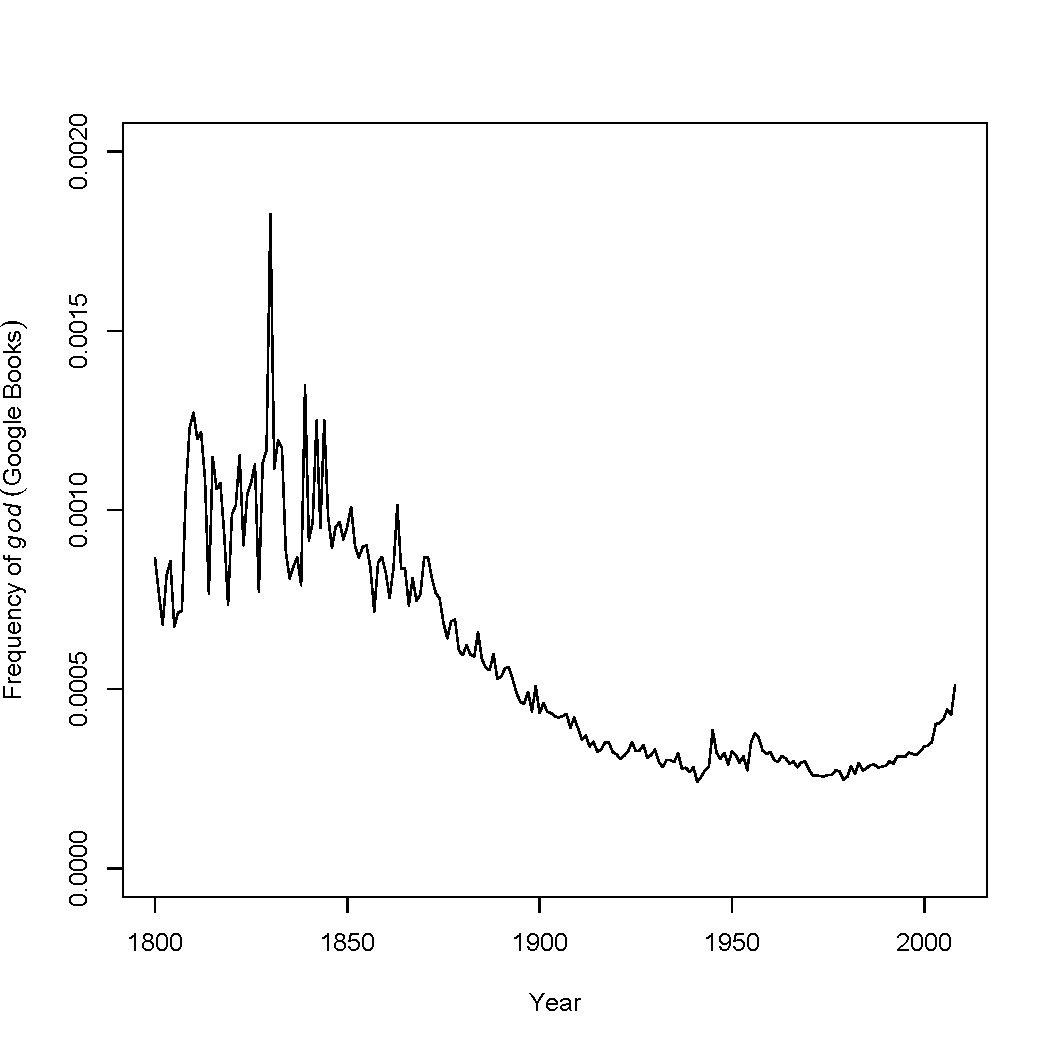
\includegraphics[width=.5\linewidth,trim=0 0 0 50]{figures/demiseofgodgoogle}%
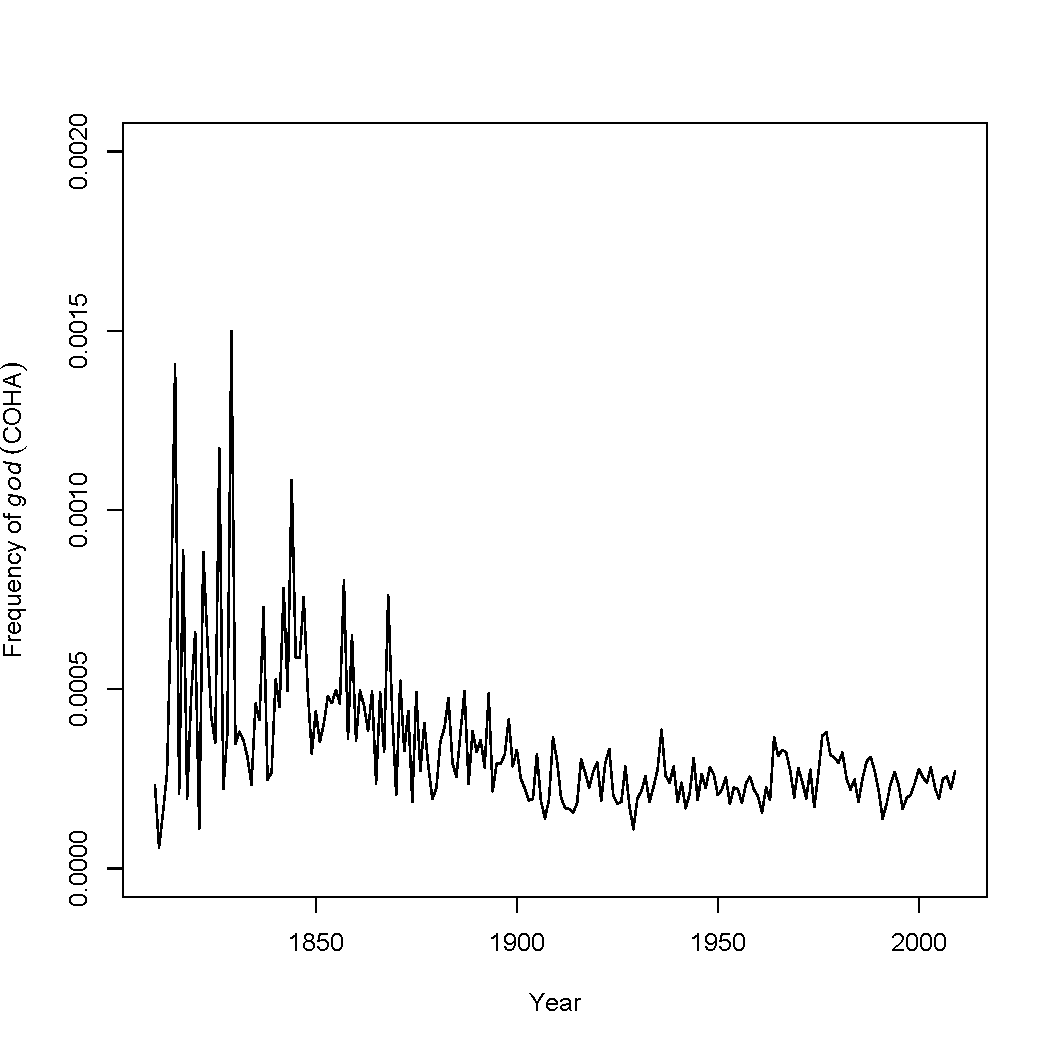
\includegraphics[width=.5\linewidth,trim=0 0 0 50]{figures/demiseofgodcoha}%
\end{figure}

Clearly, the word \textit{God} has decreased in frequency \is{frequency} -- dramatically so in the Google Books archive, slightly less dramatically so in COHA. \is{COHA} The question is what conclusions to draw from this. The authors present it as an example of the ``history of religion'', concluding from their result somewhat flippantly that ```God' is not dead but needs a new publicist''. This flippancy, incidentally, signals an unwillingness to engage with their own results in any depth that is not entirely untypical of researchers in \is{culturomics} culturomics.

Broadly speaking the result certainly suggests a waning dominance of religion on topic selection in book publishing (Google Books), and slightly less so in published texts in general (COHA). \is{COHA} This is not surprising to anyone who has paid attention for the last 200 years; more generally, it is not surprising that the rise and fall in importance of particular topics is reflected in the frequency \is{frequency} of the vocabulary used to talk and write about these topics, but the point of this case study was mainly to demonstrate that the method works.

While it is not implausible to analyze culture \is{culture} in general on the basis of a literary \is{literary language} corpus, any analysis that involves the area of publishing itself will be particularly convincing. One such example is the use of frequencies \is{frequency} to identify periods of censorship in \citet{michel_quantitative_2011}. For example, they search for the name of the Jewish artist \textit{Marc Chagall} in the German and the US\hyp{}English corpora. As \figref{fig:marcchagall} shows, there is a first peak in the German corpus around 1920, but during the time of the Nazi government, the name drops to almost zero while it continues to rise in the US\hyp{}English corpus.

\begin{figure}
\caption{The name \textit{Marc Chagall} in the US\hyp{}English and the German parts of the Google Books corpus}
\label{fig:marcchagall}
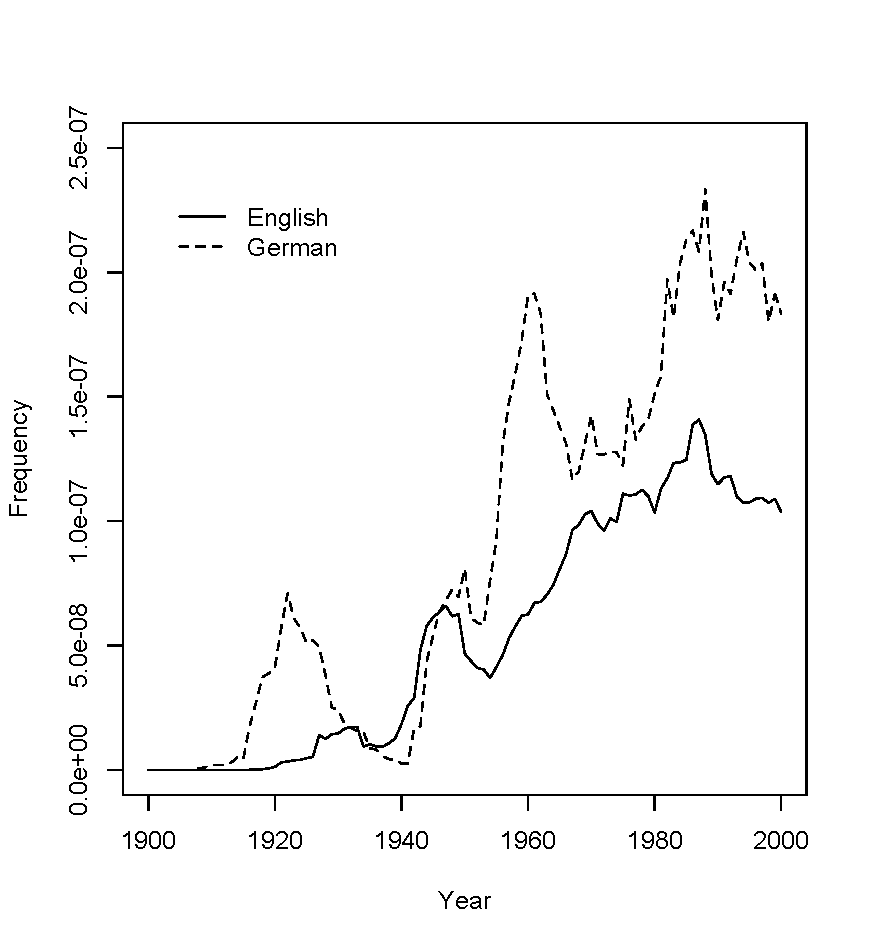
\includegraphics[width=.75\textwidth,keepaspectratio,trim=0 0 0 50]{figures/chagallcensored}
\end{figure}

The authors plausibly take this drastic drop in frequency \is{frequency} as evidence of political censorship -- Chagall's works, like those of other Jewish artists, were declared to be ``degenerate'' and confiscated from museums, and it makes sense that his name would not be mentioned in books written in Nazi Germany. However, the question is, again, what conclusions to draw from such an analysis. Specifically, we know how to interpret the drop in frequency \is{frequency} of the name \textit{Marc Chagall} during the Nazi era in Germany because we know that Marc Chagall's works were banned. But if we did not know this, we would not know how to interpret the change in frequency, since words, especially names, may rise or fall in frequency for all kinds of reasons.

Consider the following figure, which shows the development of the frequency \is{frequency} of the name \textit{Karl Marx} in the German and English Google Books archive (extracted from the bigram \is{bigram} files downloaded from the Google Books site, see Supplementary Online Material, file CUBF). Note the different frequency scales -- the name is generally much more frequent in German than in English, but what interests us are changes in frequency.

\begin{figure}
\caption{The name \textit{Karl Marx} in the English and the German parts of the Google Books corpus}
\label{fig:karlmarx}
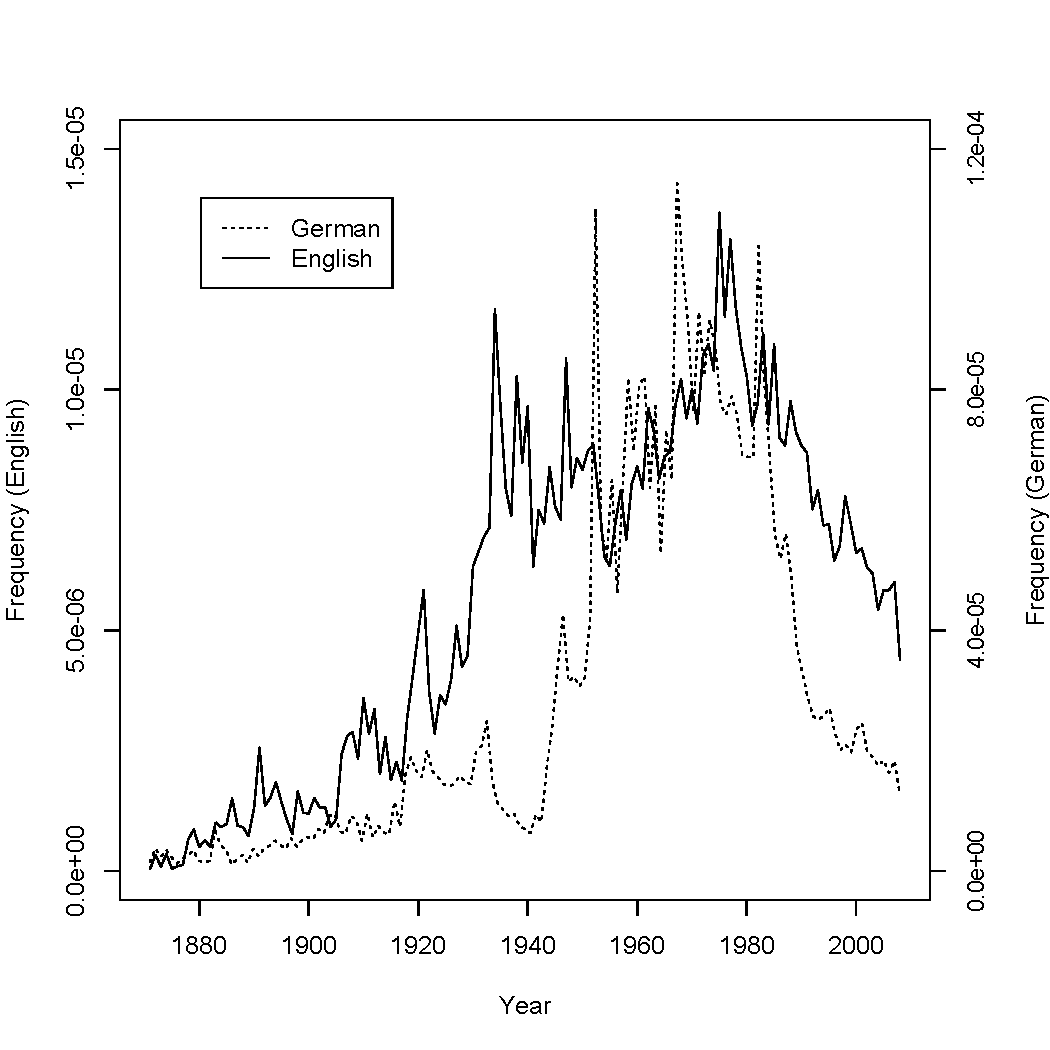
\includegraphics[width=.75\textwidth,keepaspectratio,trim=0 0 0 50]{figures/karlmarx}
\end{figure}

Again, we see a rise in frequency \is{frequency} in the 1920s, and then a visible decrease during the Nazi era from 1933 to 1945. Again, this can plausibly be seen as evidence for censorship in Nazi Germany. Plausibly, because we know that the Nazis censored Karl Marx's writings -- they were among the first books to be burned in the Nazi book burnings of 1933. But what about other drops in frequency, both in English and in German? There are some noticeable drops in frequency in English: after 1920, between 1930 and 1940 (with some ups and downs), and at the beginning of the 1950s. Only the latter could plausibly be explained as the result of (implicit) censorship during the McCarthy era. Finally, the frequency \is{frequency} drops massively in both languages after 1980, but there was no censorship in either speech community. A more plausible explanation \is{explanation} is that in the 1980s, neoliberal capitalism became a very dominant ideology, \is{ideology} and Marx's communist ideas simply ceased to be of interest to many people (if this explanation is correct, we might see the frequency of the name rise again, given the current wide\hyp{}spread disillusionment with neoliberalism).

Thus, the rise and fall in frequency \is{frequency} cannot be attributed to a particular cause without an investigation of the social, economic and political developments during the relevant period. As such, culturomics \is{culturomics} can at best point us towards potentially interesting cultural changes that then need to be investigated in other disciplines. At worst, it will simply tell us what we already know from those other disciplines. In order to unfold their potential, such analyses would have to be done at a much larger scale -- the technology and the resources are there, and with the rising interest in \textit{digital humanities} \is{humanities} we might see such large\hyp{}scale analyses at some point.
